\minitoc

\vfill

Presented herein is a detailed tour of the different notions necessary for the understanding of the present manuscript.
It is divided into three sections.
First, we categories, in Section~\ref{sec::state_of_the_art::building_modeling}, the building \gls{acr::3d} modeling techniques.
A global idea of the subject is required to have a good idea of what defects to expect in evaluated building models.
Second, we present a complete state-of-the-art survey on quality evaluation for \gls{acr::3d} building models (\textit{cf.} Section~\ref{sec::state_of_the_art::quality}).
In the last Section~\ref{sec::state_of_the_art::mlpr}, are presented the main tools that are used in our proposed approach.
Indeed, we discuss aspects of supervised classification as well as some feature extraction techniques.

\clearpage

\section{\textsc{Building \texorpdfstring{\gls*{acr::3d}}{3D} modeling}}
    \label{sec::state_of_the_art::building_modeling}
    The goal of this section is to present a general prespective on \gls{acr::3d} modeling techniques.
    This is not in any case a complete survey of this field.
    We refer the reader to a comprehensive study of metods used in urban reconstruction by~\textcite{musialski2013survey}.\\
    Herein, we classify the building modeling approaches based on different criteria.
    In Section~\ref{subsec::state_of_the_art::building_modeling::input}, we discuss the different types of input data fed to modeling pipelines.
    Next, in Section~\ref{subsec::state_of_the_art::building_modeling::automation}, is presented the different levels of automation in proposed \gls{acr::3d} modeling, while in Section~\ref{subsec::state_of_the_art::building_modeling::strategy}, are discussed the different modeling strategies.
    We finish by mentioning the differences between outdoor and indoor modeling in Section~\ref{subsec::state_of_the_art::building_modeling::in_out_door}, as well as the scalability of the different techniques.

    \subsection{\textsc{Input data heterogenuity}}
        \label{subsec::state_of_the_art::building_modeling::input}
        
        \subsubsection{\textsc{Acquisition mode}}

        \subsubsection{\textsc{Data type}}

    \subsection{\textsc{Automation level}}
        \label{subsec::state_of_the_art::building_modeling::automation}

    \subsection{\textsc{Modeling strategy}}
        \label{subsec::state_of_the_art::building_modeling::strategy}

    \subsection{\textsc{Indoor \textit{vs.} Outdoor}}
        \label{subsec::state_of_the_art::building_modeling::in_out_door}

    \subsection{\textsc{Modeling pipeline scalability}}
        \label{subsec::state_of_the_art::building_modeling::scalability}

    \clearpage
\section{\textsc{Quality evaluation of \texorpdfstring{\gls*{acr::3d}}{3D} building models}}
    \label{sec::state_of_the_art::quality}
    We have seen previously the various methods used to automatically model buildings.
    The goal of this section is to describe the available approaches that evaluate the quality of such models.
    These could be distinguished based on two criteria.\\
    In Subsection~\ref{subsec::state_of_the_art::quality::output}, are presented the quality evaluation methods based on their output.
    An alternative perspective to charecterize quality evaluation methods relies upon the type of reference data (\textit{cf.} Subsection~\ref{subsec::state_of_the_art::quality::reference}).
    Based on this survey, we state in details, in Subsection~\ref{subsec::state_of_the_art::quality::novelty}, how the work presented in this thesis is different from what was already proposed in the literature. 

    \subsection{\textsc{Output types}}
        \label{subsec::state_of_the_art::quality::output}
        We distinguish herein quality evaluation methods based on the kind of output they produce.
        Fidelity metrics is a first instance of output types.
        The second is semantic labels.
        In what follows, we explain, in details, these differences between the two method types.

        \subsubsection{\textsc{Fidelity metrics based methods}}
            One way to characterize the quality of a building model is to compute indices or metrics reporting its accuracy.\\

            Most metrics provide information on the geometric precision of the model.
            These are computed for different geometric objects.
            Below, depending on the geometric dimension of the latter, we categorize the geometric fidelity metrics.\\

            We start with zero dimensional objects: \textit{i.e.} points.
            In this case, metrics are based on their coordinates.
            The goal is to detect positional inaccuraccies~\parencite{kaartinen2005accuracy}.
            In constrast, the choice of points to be inspected is not simple.
            Corner points resulting from the intersection of edges in the model is one choice.
            In fact,~\textcite{zeng2014multicriteria} registers corner points from the evaluated model and the corresponding reference.
            Based on this registration, a comparison is drawn using \gls{acr::rmse}, just as in~\parencite{landes2012quality} and~\parencite{you2011quality}.
            The same points are used as a proxy for manual quality inspection by~\textcite{elberink2011quality}.
            Another alternative is to sample points from lines or surfaces to be compared.
            These could be predetermined manually as in~\textcite{kaartinen2005accuracy} or sampled regularely as demonstrated by~\textcite{vogtle2003quality} or by~\textcite{tran2019geometric}.
            Imprecisions are not computed only relying the \gls{acr::rmse}, but can also be separated into planimetric and height inaccuraccies~\parencite{vogtle2003quality, kaartinen2005accuracy, jaynes2003recognition}.\\

            Second comes edges and all one dimensional objects in general.
            These convey structural, in addition to positional, informations.
            \textcite{kaartinen2005accuracy} compares lengths as well as slopes of edges formed by reference points.
            Edges related metrics are also used as an intermediary as shown by~\textcite{elberink2011quality} and~\textcite{michelin2013quality}.
            They are both interested in edges resulting from facet intersections.
            While the first relies on \gls{acr::rmse}, the second computes more complex metrics that compares model edges to ones extracted out of sensor data.\\

            Next are compared surfaces (\textit{i.e.} two dimensional objects), bounded (for example, polygons) or not (like planes).
            These hold more structural information than the first ones and hence are widely used for evaluation.
            \textcite{rottensteiner2014results} used height discrepency of roof planes so as to evaluate building models.
            This ideal for Manhattan-world assumptions as was the case of~\textcite{zebedin2008fusion}.
            In addition to height discrepency, normal displacement is computed using always the same \gls{acr::rmse} metric by~\textcite{henricsson19973}.
            Conversely,~\textcite{zeng2014multicriteria} uses also a \gls{acr::rmse} for comparison, but not in the Euclidean space.
            In fact, after mapping the evaluated and reference models to a sphere, they compare their spherical harmonic~\parencite{brechbuhler1995parametrization} representations.
            Just as with edges, planes can be evaluated using angular measurements, as was proposed by~\textcite{landes2012quality} and~\textcite{henricsson19973}.
            Another alternative is to compare reconstructed and reference models based on surface area comparisons.
            These are mostly based on ratios like completeness and correctness\footnote{in other words, recall and precision respectively.}~\parencite{rottensteiner2014results,landes2012quality,henricsson19973,schuster2003new}.\\

            Last, are three dimensional (\textit{i.e.} volume) evaluation.
            The same detection ratios that were computed for surfaces are again calculated to evaluate volumes this times, as shown by~\textcite{mohamed2013quality, zeng2014multicriteria,jaynes2003recognition,nguatem2017modeling}.
            These are the only metrics used for volumes that we are aware of.\\

            Regarding \textit{implicit} semantics, as far as we are aware, only one metric is widely used to evaluate its impact.
            As discussed previously in Subsection~\ref{subsec::introduction::urban_3d_reconstruction::building_3d_modeling}, compaction is one byproduct of semantics.
            As a consequence, it was used as an index to evaluate reconstructions\footnote{It is sometimes called by its antonym: complexity.}: the more a model was compact the better it was.
            This is reflected, for instance, in the work of~\textcite{lafarge2012creating},~\textcite{zhang2017deep},~\textcite{duan_eccv16},~\textcite{zeng2018neural} and~\textcite{zhu2018large}, where this metric is never used alone but always alongside geometric ones.

        \subsubsection{\textsc{Semantic labels based methods}}
            \label{subsec::state_of_the_art::quality::output::semantic}
            In a drive to provide a quantitative assessment of building models, the previously defined metrics fail to convey specific and localized information about a predetermined building model.
            These indices are usually used to give a general idea of the quality of models produced by some modeling method.
            Moreover, they do not usually carry semantics, which is critical for further processing steps such as manual correction~\parencite{elberink2011quality}.
            Some evaluation methods, in an effort to alleviate these issues, yield semantic labels that describe the errors of an evaluated model.
            Hereafter, are described the different types of labels that were proposed in the literature.\\

            \parencite{boudet2006supervised} was the first ever work, that we are aware of, which tackles semantic labels as outputs of the evaluation .
            This approach has four classes which indicate how much valid can the modeling be: ``acceptable'' and ``correct'' portray valid buildings while ``false"``and ``generalized"``are refused.
            It can be seen as a four grade based score system expressing the confidence in a building model.
            The main limitation of this method is the fact that the proposed labels do not specify what defects a model presents if it is not valid.
            It is, therefore, hard to use for model correction.
            Besides, the acceptable defect definitions depend also on each use case.
            For instance, a comunications company would be more adament on the accuracy of roof parts, which would affect wave propagation, rather than an insurance company interested in flood damage estimation.
            This means that each use case implies a relabeling that could be potentially different from other one.\\
            
            The first hints of a fine grained semantic labeling of building model errors lay in the work of~\textcite{rottensteiner2014results}.
            This work was the first to report segmentation issues, at facet level, in labels instead of a global ratio.
            They distinguish between oversegmentation cases, undersegmentation cases and cases where both co-occur.\\

            On the other hand, these mentioned errors are not comprehensive: they do not cover all possible building model errors.
            \textcite{michelin2013quality} came up with a richer taxonomy of errors that are categorized into three big families:
            \begin{itemize}
                \item Footprint errors: these portray errors relative to the building footprint, which is used by many modeling algorithms as input.
                        Errors contained in this family are: ``erroneous outline'', ``unexisting building'', ``missing inner court'' and ``inaccurate footprint''.
                \item Reconstruction errors: these are caused by the modeling approach.
                        These defects can be the result of the incompatibility of some \textit{a priori} hypotheses about the scene, for instance.
                        Such errors are: ``under-segmentation'', ``over-segmentation'', ``inaccurate roof'' and ``Z translation''.
                \item Vegetation errors: this corresponds to a special case when modeled building are occluded, completely or partially, by higher vegetation.
                        It becomes impossible to evaluate properly these models.
            \end{itemize}
            Although the last taxonomy is rich, it is not exhaustive enough as it misses cases that are not present in the urban zone that was studied in the paper, such as inaccurate primitive choices.
            Moreover, it adopts the point of view of the modeling method that was used to provide their dataset.
            Knowing the specific weaknesses of the latter guided the choice of error family classification and the error definitions.
            This is particularly clear when looking at their error categorization.
            In fact, the first error class relates to the fact that the used building modeling approach~\parencite{durupt2006automatic} relies on footprints given as input.
            The second category corresponds to the actual step of building roof structure inference.

    \subsection{\textsc{Reference data types}}
        \label{subsec::state_of_the_art::quality::reference}
        In order to evaluate models, reference data are utilized for comparison.
        Based on the latter, another way to discriminate among modeling methods is possible.
        The first class of reference data are high quality ground truth building \gls{acr::3d} models.
        Remote sensing data is the second alternative that is used for reference.
        Neither of these two choices do influence the type of output the evaluation method produces.
        Hereafter, is explained the difference between the two categories.

        \subsubsection{\textsc{High resolution ground truth}}
            Ground truth building models are mainly acquired manually.
            Herein, are listed the different ground truth measurement techniques, in descending order of accuracy.\\

            The most obvious case consists in field measurements of the modeled building.
            \textcite{dick2004modelling}, for instance, evaluated their buildings based on manual tape measurements taken on specific architectural features, like windows and columns, with an accuracy of \SI{0.01}{\m} for the first and \SI{0.1}{\m} for the second.
            Complete and scalables measurements of buildings are possible using topographic surveys.
            Using the latter, building models could be reconstructed with precision up to \SI{\pm 0.1}{\m}~\parencite{henricsson19973} or \SI{\pm 0.05}{\m}~\parencite{vogtle2003quality}.\\
            There is also the possibility of manually modeling the building using oblique images, or stereoplotting.
            ~\textcite{zebedin2008fusion} uses such a method to produce their reference data from aerial images with accuracy up to the order of \SI{\pm 0.15}{\m}.
            The same procedure was used also by~\textcite{jaynes2003recognition} producing models with inaccuraccies bounded by \SI{\pm 1/3}{\m}.

        \subsubsection{\textsc{Remote sensing data}}
            Reference ground truth models are not easy to come by~\parencite{schuster2003new}.
            The previous choice is hard to scale up to district or city levels.
            In fact, they are more suitable to evaluate few building models: \textit{e.g.} in order to validate a reconstruction method.
            On the other hand, remote sensing data are more accessible and could be used, instead, as reference.
            In fact, since these are usually fed as input in modeling methods, it is only reasonable to evaluate the produced models in comparison to the intake.
            Listed here, are the different types of remote sensing data and how they could be used for building model evaluation.\\

            Aerial images are the first example of reference data used in building model evaluation.
            These could be original oblique images or preprocessed orthoimages.
            The first class of images are the most precise but the other one is more available.
            Oblique images were used by~\textcite{michelin2013quality} to extract \gls{acr::3d} segments based on plane sweeping techniques.
            Reference edges are filtered out and are used to evaluate the \gls{acr::3d} model (intersection) edges.
            Based on these segments,~\textcite{boudet2006supervised} not only evaluates edges but also corners (\textit{i.e.} edge intersections) and planes.
            Facet were also evaluated, in~\parencite{boudet2006supervised}, based on correlation functions computed from multiple overlapping oblique images.
            Orthoimages were used also to, for instance, compute \gls{acr::ndvi} scores for vegetation occluded building model discrimination.\\

            Second, are \gls{acr::lidar} point clouds.
            This type of data have the inherent advantage, compared to images, of natively providing depth information.
            \textcite{kaartinen2005accuracy} used data that was acquired multiple times with a guarantied precision up to \SI{0.083}{\m} in plane and \SI{0.035}{\m} in height.
            Out of the latter were chosen reference points that were compared to equivalents in the evaluated building models (check the previous sub-subsection).
            All the points could also be used for comparison by computing metrics such as \gls{acr::rmse}~\parencite{lafarge2012creating,zhu2018large}.
            Original input data is not always accessible.
            One issue arises when using different data: data registration.
            This is taken into account by~\textcite{akca2010quality}, before addressing the completeness of building models.\\
            
            Third and last, are presented height maps.
            These are not sensor data as they are a byproduct of earlier data types.
            Still, they are considered here since they are used as input by some building modeling pipelines.
            Just like with \gls{acr::lidar}, \gls{acr::dsm} is used for building models comparison based on \gls{acr::rmse}~\parencite{zeng2018neural}.
            \textcite{michelin2013quality}, however, uses the same data but differently.
            In fact, \gls{acr::dsm}, being a result of oblique images, can be used as proxy, to help extracting \gls{acr::3d} geometric features instead of recomputing correlation scores like in~\parencite{boudet2006supervised}.
            It can also be valuable for missing court detection by calculating sky viewshed angle scores~\parencite{michelin2013quality}.

    \subsection{\textsc{Novelty of the proposed method}}
        \label{subsec::state_of_the_art::quality::novelty}
        Based on the Subsection~\ref{subsec::introduction::contributions::positioning}, we can understand how most quality evaluation methods are unsuitable for the objectives that where stated.\\

        In fact, the semantic character of the evaluation overrules approaches relying only on geometry based metrics.
        This represents most of the methods discussed earlier (\textit{c.f.} Subsection~\ref{subsec::state_of_the_art::quality::output}).
        These metrics could be used afterwards one a semantic error is identified as a complement to help quantify the defect.
        On the other hand, the need for reasonably available reference data, which is dictated by the large-scale constraint, implies the reliance on remote sensing data based methods (\textit{c.f.} Subsection~\ref{subsec::state_of_the_art::quality::reference}).\\

        Methods that satisfy both conditions are in the number of two:~\textcite{boudet2006supervised,michelin2013quality}.
        Both define semantic errors that are detected using Oblique images and \glspl{acr::dsm}.
        A classifier learns statistical properties of the building \gls{acr::3d} models using features that are derived from these sensor data.
        The learning process further helps scaling the process to unseen data by predicting errors using the same attributes.\\

        Our work relies on the same idea, but goes a bit farther by proposing the possibility to evaluate building models without using any reference data.
        It also offers a new taxonomy of errors that is intended to be exhaustive and generalizable.
        The last idea will be developped in details in Chapter~\ref{chap::semantic_evaluation}, while Chapter~\ref{chap::learned_evaluation} presents how features are chosen to represent building models and the learning process.

\section{\textsc{Supervised learning and pattern recognition}}
    \label{sec::state_of_the_art::mlpr}
    In this section are presented notions from statistic learning and computer vision domains that were usefull for this work.
    This constitutes a simple reminder and is not a thorough survey of the field.
    Section~\ref{subsec::state_of_the_art::mlpr::classifiers} start off with a brief description of utilized supervised classifiers in .
    Second (section~\ref{subsec::state_of_the_art::mlpr::feature_extraction}) comes a presentation of computer vision concepts on which our method is based.
    Last is discussed graph classification that was also instrumental in this work.

    \subsection{\textsc{Supervised classifiers}}
        \label{subsec::state_of_the_art::mlpr::classifiers}
        In this subsection, we denote a family of observations and their classes by
        \begin{equation*}
            \left((\bm{x^i}, y^i)\right)_{i=1,2,\dots,n}.
        \end{equation*}
        Features are in practice finite dimensional vectors:
        \begin{equation*}
            \forall i=1,2,\dots,n \;, \bm{x^i} \in \mathbb{R}^d.
        \end{equation*}
        Classes are modeled by a finite set bijective to the set \(\left\{1,2,\dots,C\right\}\):
        \begin{equation*}
            \forall i=1,2,\dots,n \;, y_i \in \left\{1,2,\dots,C\right\}            
        \end{equation*}
        The goal of supervised classification is to learn, based on the training set $\left((\bm{x^i}, y^i)\right)_{i=1,2,\dots,n}$, some statistical characteristics in order to predict the classes of some new observations:\footnote{This family is called the test set.}
        \begin{equation*}
            \left(\bm{x^i}\right)_{i=1,2,\dots,n'}.
        \end{equation*}
        This type of problems is said to be multi-class: each instance has one possible class out of a number of possibilities.
        In the special case of binary classification, only two classes are possible:
        \begin{equation*}
            \forall i=1,2,\dots,n \;, y^i \in \left\{0, 1\right\}
        \end{equation*}
        
        On another hand, the multi-label classification problem is the case where to each instance corresponds a number $L$ of binary labels:
        \begin{equation*}
            \forall i=1,2,\dots,n \;, y^i = (y^i_1, y^i_2, \dots, y^i_L) \in \left\{0, 1\right\}^L.
        \end{equation*}
        In this case, associating features with each label \(\left(\left(\bm{x^i}, y^i_l\right)\right)_{i=1,2,\dots,n}\) can be seen as an independent binary classification problem.
        This is different from multi-class problems, as for the latter only one class is possible while in the other multiple labels can be detected per instance.\\

        Hereafter, are presented two supervised classifiers: the \gls{acr::svm} algorithm and Random Forests, both of which are used in this work.

        \subsubsection{\textsc{\acrlong*{acr::svm}}}
            \label{subsubsec::state_of_the_art::mlpr::classifiers::svm}
            \glspl{acr::svm} are a special type of linear classifiers.
            The initial classes $\left(y^k\right)_{k=1, 2, \dots, n}$ are transformed into $\left(\tilde{y}^k\right)_{k=1, 2, \dots, n}$, using the map: $y \mapsto \tilde{y} = 2\cdot y - 1$.
            There are always two possible classes $\left\{1, -1\right\}$.
            This simple transformation is use so as to simplify the latter equations.

            We remind the reader of the decision function\footnote{A decision function assigns a class to given observation.} of a linear classifier:
            \begin{equation}
                \label{eq::linear}
                \begin{aligned}
                    \mathbf{D}_{\text{linear}, \bm{w}, b}: \mathbb{R}^d &\rightarrow \left\{-1, 1\right\}\\
                    \bm{x} &\mapsto 2 \cdot \mathbb{1}_{\bm{w}^\intercal \cdot \bm{x} + b\geq 0} - 1 \quad.
                \end{aligned}
            \end{equation}
            where:
            \begin{conditions}
                \bm{w} & is the weight vector;\\
                b & is the bias.
            \end{conditions}

            \paragraph{Hard margin}
                In order to understand the idea behind the \gls{acr::svm} classifier, we start by assuming that the dataset to be classified $\left((\bm{x}^k, y^k)\right)_{k=1, 2, \dots, n}$ is linearly separable.
                It means that there is at least one hyperplane $(H_0)$ that can separate perfectly the two classes.
                We can order points of one class based on their distance to the hyperplane $(H_0)$: $\bm{x} \mapsto d(\bm{x}, H_0)$.
                The closest positive (\textit{resp.} negative) points (\textit{i.e.} of class $1$ (\textit{resp.}  $-1$)) to $(H_0)$ are called positive (\textit{resp.} negative) support vectors.
                Support hyperplanes are the hyperplanes that are parallel to the separator and passes through the support vectors.
                This can be summarized as:
                \begin{eqnarray}
                    \left\{\bm{x}^+_s: s = 1, 2, \dots, n_{psp}\right\} &\triangleq \arg\min\left\{d(\bm{x}_k, H_0) : k=1, 2, \dots, n \wedge \tilde{y}^k = 1\right\}\\
                    \left\{\bm{x}^-_s: s = 1, 2, \dots, n_{nsp}\right\} &\triangleq \arg\min\left\{d(\bm{x}_k, H_0) : k=1, 2, \dots, n \wedge \tilde{y}^k = -1\right\}
                \end{eqnarray}
                where:
                \begin{conditions}
                    n_{psp} & is the number of positive support vectors.\\
                    n_{nsp} & is the number of negative support vectors.\\
                \end{conditions}

                We define:
                \begin{equation*}
                    Sol \triangleq \left\{\omega \in \mathbb{R}^d : \omega.\bm{x} + b = 0\right\}.
                \end{equation*}
                We verify that:
                \begin{equation*}
                    \forall \lambda \in \mathbb{R}\setminus\left\{0\right\}, \; (\bm{w}, b) \in  Sol \Leftrightarrow (\lambda . \bm{w}, \lambda.b) \in Sol.
                \end{equation*}
                In other words, the solution $(\bm{w}^*, b^*)$ is unique up to multiplicatif term $\lambda \in \mathbb{R}\setminus\left\{0\right\}$.
                In this context, $(\bm{w}, b)$ is chosen so that \(\bm{w}\) points to the positive instances\footnote{The positive instances are inside the positive half-space.} and the support hyperplanes verify:
                \begin{equation}
                    \label{eq::support_lines}
                    \begin{cases}
                        \forall s=1,2,\dots,n_{psp} \quad \bm{w}^\intercal\cdot\bm{x}^+_s + b = 1\\              
                        \forall s=1,2,\dots,n_{nsp} \quad \bm{w}^\intercal\cdot\bm{x}^-_s + b = -1                
                    \end{cases}
                \end{equation}

                \begin{figure}
                    \centering
                    \includestandalone[mode=buildnew, width=\textwidth]{figures/svm/linear_separable}
                    \caption[
                        Illustration of the hard-margin \acrshort*{acr::svm}.
                    ]{
                        \label{fig::linear_separable} 
                        Illustration of the hard-margin \gls{acr::svm}.
                        A hyperplane separator in $\mathbb{R}^2$ corresponds to a line.
                        In this case, $n_{psp} = n_{nsp} = 1$.
                        The support lines are plotted in orange.
                        $M$ is the margin.
                    }
                \end{figure}

                Figure~\ref{fig::linear_separable} illustrates these notions.
                The uncertainty of a point classification is an increasing function of the distance of that point to the separator.
                In the hard margin case, the given samples are supposed to be certain.
                Since support vectors are the closest certain points to $(H_0)$, the class of points $\bm{p}$ that verify $\vert\bm{w}^\intercal\cdot\bm{p} + b\vert \geq 1$ is known with probability $1$.
                Conversely, the points that lay between the support hyperplanes are the most uncertain.
                The bigger the distance between these two lines the more nuanced the classifier decision is.
                The main idea behind \glspl{acr::svm} is to maximize this distance.
                It is called margin and denoted $M$.\\

                In order to compute the margin, we can interpret it as the length of the orthogonal projection of any vector $\bm{v}_{st}$\footnote{$\forall (s, t) \in \left\{1,2,\dots,n_{nsp}\right\} \times \left\{1,2,\dots,n_{psp}\right\}$} going from a negative support vector $\bm{x}^-_s$ to a positive one $\bm{x}^+_t$ on any line carried by $\bm{w}$.
                Since all support vectors of the same class lay on the same line, the choice of $(s,t)$ is inconsequential.
                We can hence deduce:
                \begin{align}
                    M &= \frac{\bm{w}^\intercal}{\Vert\bm{w}\Vert} \cdot (\bm{x}^+_1 - \bm{x}^-_1) \nonumber \\
                    M &= \frac{2}{\Vert\bm{w}\Vert}
                \end{align}

                Maximizing $M$ is actually equivalent to minimizing $\Vert\bm{w}\Vert$.
                In the purpose of simplifying the resolution of the problem, we drop the square root and minimize instead $\Vert\bm{w}\Vert^2$.
                The certainty in the given samples is translated by the inequalities:
                \begin{equation*}
                    \begin{cases}
                        \bm{w}^\intercal\cdot\bm{x}^i + b \geq 1 & \forall i \in \left\{1, 2, \dots, n: \tilde{y}^i = 1\right\}\\
                        \bm{w}^\intercal\cdot\bm{x}^i + b \leq -1 & \forall i \in \left\{1, 2, \dots, n: \tilde{y}^i = -1\right\}
                    \end{cases}.
                \end{equation*}
                These can be summed in one, as follows:
                \begin{equation}
                    \label{eq::hard_margin}
                    \tilde{y}^i.(\bm{w}^\intercal\cdot\bm{x}^i + b) \geq 1 \; \forall i = 1, 2, \dots, n.
                \end{equation}
                Thus, the \gls{acr::svm} problem can be formalized as a convex constrained quadratic optimization one:
                \begin{equation}
                    \label{eq::hard_svm_primal}
                    \begin{aligned}
                        & \min_{\bm{w}}
                        & & {\Vert \bm{w} \Vert}^2 \\
                        & \text{s.t.}
                        & & \tilde{y}^i.(\bm{w}^\intercal\cdot\bm{x}^i + b) \geq 1 \; \forall i = 1, 2, \dots, n
                    \end{aligned}.
                \end{equation}

            \paragraph{Soft margin}
                In the previous case, we assumed that we are always certain about the classes of the given samples.
                The margin cannot contain any of those points.
                This explains the name hard margin.
                We are always guaranteed to have a solution of a hard margin \gls{acr::svm} in the case of linear separability.
                however, if the last condition is not met, there is no such solution.
                To alleviate this problem,~\textcite{cortes1995support} allowed some uncertainty in the given samples in order to fit the linear model.\\

                \begin{figure}
                    \centering
                    \includestandalone[mode=buildnew, width=\textwidth]{figures/svm/non_linear_separable}
                    \caption[
                        Illustration of a soft margin \acrshort*{acr::svm}.
                    ]{
                        \label{fig::soft_margin} Illustration of a soft margin \gls{acr::svm}.
                        The orange lines (\textit{resp.} green line) correspond to the support hyperplanes (\textit{resp.} separator).
                        Dataset points are allowed to be inside the margin and even in the other side of the separator.
                        It helps fit a natively linear classifier in a non linearly separable case.supervised classification
                    }
                \end{figure}

                To put this into mathematical terms, we start by the reminding the constraint of the hard margin problem in Equation~\ref{eq::hard_margin}.
                Allowing uncertainty for some given point $\bm{x}^i$ comes back to allowing it to be in the wrong side of the support hyperplane: \textit{i.e.} $\tilde{y}^l.(\bm{w}^\intercal\cdot\bm{x}^l + b) < 1$.
                In this case, we define: $\xi^i := 1 - \tilde{y}^i.(\bm{w}^\intercal\cdot\bm{x}^i + b) > 0$.
                Otherwise, $\xi^i := 0$.
                These defined values are called slack variables.
                They express how much each point is uncertain.
                They can be expressed in a compressed form called hinge loss:
                \begin{equation}
                    \label{eq::slack_variables}
                    \xi^i \triangleq \max\left(1 - \tilde{y}^i.(\bm{w}^\intercal\cdot\bm{x}^i + b), 0\right).
                \end{equation}
                The soft margin constraint translates now to:
                \begin{equation}
                    \label{eq::soft_margin}
                    \tilde{y}^i.(\bm{w}^\intercal\cdot\bm{x}^i + b) \geq 1 - \xi^i.
                \end{equation}
                Four cases are distinguished, for slack variables:
                \begin{itemize}
                    \item $\xi^i = 0$: the class of the point is certain;
                    \item $0 < \xi^i \leq 1$: the point is of the same class but is uncertain: \textit{i.e.} between the support hyperplane and the separator;
                    \item $1 < \xi^i < 2$: the point is of the opposite class and is uncertain: \textit{i.e.} between the separator and the opposite support hyperplane;
                    \item $2 \leq \xi^i$: the point is certainly of the opposite class: \textit{i.e.} beyond the opposite support hyperplane.
                \end{itemize}
                As a consequence, when a dataset is not linearly separable, at least one sample $i_0$ cannot fit in a linear model and $1 < \xi^{i_0}$.
                All these situations are illustrated in Figure~\ref{fig::soft_margin}.\\

                The idea is to find a configuration where most slack variables are null or near $0$.
                Sparsity is also wished: we prefer having one wrong point rather than a lot of points that are uncertain.
                For this purpose, these variables would be penalized against using an $L_1$ norm.
                Since all slack variables are positive, the soft margin \gls{acr::svm} problem becomes:
                \begin{equation}
                    \label{eq::soft_svm_primal}
                    \begin{aligned}
                        & \min_{\bm{w} \in \mathbb{R}^d}
                        & & {\Vert \bm{w} \Vert}^2 + C \cdot \sum_{i=1}^n \xi^i \\
                        & \text{s.t.} & & \tilde{y}^i.(\bm{w}^\intercal\cdot\bm{x}^i + b) \geq 1, \; \forall i = 1, 2, \dots, n\\
                        & & & \xi^i \geq 0, \; \forall i = 1, 2, \dots, n
                    \end{aligned}.
                \end{equation}
                where:
                \begin{conditions}
                    C & is the penalization constant.\\
                \end{conditions}

                A small $C$ means the slack variables are allowed to get big: the margin is expected to be big.
                A high $C$ leads to a tight margin as it penalizes any uncertainty.
                The special case where $C=\infty$ corresponds simply to the hard margin case.
                Hence, the penalization constant is tuned, using cross-validation for instance, so as to achieve the best generalization power.

                Since the problem stated in Equation~\ref{eq::soft_svm_primal} is a convex optimization problem, solving it is equivalent to solving the dual:
                \begin{equation}
                    \label{eq::soft_svm_dual}
                    \begin{aligned}
                        & \max_{\alpha_1, \alpha_2, \dots, \alpha_n \in \mathbb{R}_+}
                        & & \sum_{1\leq i \leq n} \alpha_i - \frac{1}{2}\cdot\sum_{\substack{1\leq l \leq n\\1\leq p \leq n}}\alpha_l\cdot\alpha_p\cdot\tilde{y}^l\cdot\tilde{y}^p\cdot(\bm{x}^l)^\intercal\cdot\bm{x}^p\\
                        &\text{s.t.} & & \sum_{1 \leq i \leq n}\tilde{y}^i\cdot\alpha_i=0 \\
                        & & & 0 \leq \alpha_i \leq C \;\forall i=1,2,\dots,n
                        \end{aligned}
                \end{equation}
                A fast solution of this problem is possible using the \gls{acr::smo} developped by~\textcite{platt1998sequential}.
                This will not be detailed herein. 

            \paragraph{Kernel \acrshort*{acr::svm}}
                Not all classification problems can be solved in a linear manner.
                Unfortunately, \gls{acr::svm} is inherently linear.
                However, there is a way to generalize this classifier.\\

                \begin{figure}
                    \centering
                    \ffigbox[\FBwidth]{
                        \begin{subfloatrow}[2]
                            \ffigbox[\FBwidth]{
                                \includestandalone[mode=buildnew, width=.45\textwidth]{figures/svm/circles_original}
                            }{
                                \caption{
                                    \label{subfig::original_circles}
                                    Original representation of the dataset in the feature space.
                                }
                            }
                            \ffigbox[\FBwidth]{
                                \includestandalone[mode=buildnew, width=.45\textwidth]{figures/svm/circles_polar}
                            }{
                                \caption{
                                    \label{subfig::polar_circles}
                                    Representation of the dataset using polar coordinates
                                }
                            }
                        \end{subfloatrow}
                    }{
                        \caption{
                            \label{fig::circles_transformation}
                            Example of a transformation of a dataset that can be linearly separable in the maped space. 
                        }
                    }
                \end{figure}

                The original feature space where the data is represented is not always an ideal\footnote{An ideal space is one where distances between points are meaningful} one.
                A solution is to find a transformation $\Phi: \mathbb{R}^d \rightarrow \mathscr{H}$ that maps initial feature vectors into a Hilbert space $(\mathscr{H}, \langle\cdot{,}\cdot\rangle_{\mathscr{H}})$ where distances between instances are meaningful.
                There is no unique map that satisfy this type of properties.
                We are particularly intersted in a map which transforms the data into a space where they are hopefully linearly separable~\parencite{boser1992training}.
                This illustrated in Figure\ref{fig::circles_transformation}.
                Using a polar coordinate transformation 
                \begin{align*}
                    \Phi: \mathbb{R}^2 &\rightarrow \mathbb{R}^2 \\
                    \begin{bmatrix}
                        x \\
                        y
                    \end{bmatrix} &\mapsto \begin{bmatrix}
                        \sqrt{x^2 + y^2} \\
                        \text{arctan}_2(y, x)
                    \end{bmatrix},
                \end{align*}
                the dataset can be linearly separable.
                In this particular case, the original probability distribution is known as it was generated manually.
                Moreover, the map codomain is a vector space of the same dimension as the map domain.
                This is usually not the case: in practice, the right mapping is difficult to come by\footnote{If it exists at all.} and the codomain is usually of a higher dimension possibly infinite.
                Finding such a map involves usually heavy compuations.
                However, as we are interested in distances between dataset points, there is an easier way around.
                Using the ``kernel trick'', one can compute any distance in the target space $\mathscr{H}$ using only the scalar product:
                \begin{align}
                    \label{eq::kernel_definition}
                    k: \mathbb{R}^d \times \mathbb{R}^d &\rightarrow \mathbb{R}\\
                    (\bm{x}, \bm{y}) &\mapsto \langle\Phi(\bm{x}), \Phi(\bm{y})\rangle_{\mathscr{H}} \nonumber.
                \end{align}
                Going back to the dual optimization problem stated in Equation~\ref{eq::soft_svm_dual}, we see that only the scalar product between samples is needed.
                Assuming the existence of an adequate mapping $\Phi$, and if we substitute each point by its representation in the new space, we can rewrite, so called, kernel \gls{acr::svm}.
                \begin{equation}
                    \label{eq::kernel_soft_svm_dual}
                    \begin{aligned}
                        & \max_{\alpha_1, \alpha_2, \dots, \alpha_n \in \mathbb{R}_+}
                        & & \sum_{1 \leq i \leq n} \alpha_i - \frac{1}{2}\cdot\sum_{\substack{1\leq l \geq n\\1\leq p \geq n}}\alpha_l\cdot\alpha_p\cdot\tilde{y}^l\cdot\tilde{y}^p\cdot k(\bm{x}^l, \bm{x}^p)\\
                        &\text{s.t.} & & \sum_{1 \leq i \leq n}\tilde{y}^i\cdot\alpha_i=0 \\
                        & & & 0 \leq \alpha_i \leq C \; \forall i=1,2,\dots,n
                        \end{aligned}
                \end{equation}

                There are more theoretical details for kernels which are not discussed herein.
                For more details on the subject, one can check the work by~\textcite{aronszajn1950theory},~\textcite{vapnik2013nature} or~\textcite{shawe2004kernel}.

                \subparagraph{Usual kernels}
                    The choice of kernels is not easy.
                    Practitioners experiment with different kernel types and parameters.
                    One can engineer a kernel specific for their application.
                    However, in general, there are some usual kernel that are chosen:
                    \begin{itemize}
                        \item the native linear kernel:
                        \begin{equation}
                            \label{eq::linear_kernel}
                            k(\bm{x}, \bm{y}) = \bm{x}^\intercal \cdot \bm{y};
                        \end{equation}
                        \item the \gls{acr::rbf} kernel: for some parameter $(\gamma) \in \mathbb{R}$
                        \begin{equation}
                            \label{eq::rbf_kernel}
                            k_{\gamma}(\bm{x}, \bm{y}) = \exp{-\gamma \cdot \Vert \bm{x} - \bm{y} \Vert^2};
                        \end{equation}
                        \item the polynomial kernel: for some parameters $(c, d) \in \mathbb{R}_+ \times \mathbb{N} \setminus \left\{0\right\} $
                        \begin{equation}
                            \label{eq::polynomial_kernel}
                            k_{\gamma, c}(\bm{x}, \bm{y}) = (\bm{x}^\intercal \cdot \bm{y} + c)^d;
                        \end{equation}
                        \item the sigmoid kernel: for some parameters $(\gamma, c) \in \mathbb{R}^2$
                        \begin{equation}
                            \label{eq::sigmoid_kernel}
                            k_{\gamma, c}(\bm{x}, \bm{y}) = \gamma \cdot \tanh(\bm{x}^\intercal \cdot \bm{y} + c).
                        \end{equation}
                    \end{itemize}
                    The choice of kernel parameters in important not only for achieving good classification results but also to avoid overfitting problems.

                \subparagraph{\acrlong*{acr::mkl}}
                    Some operations over kernels always yield valid kernels.
                    This is true for instance for summation.
                    In fact, fixing the number of kernels $K\in \mathbb{N} \setminus \left\{0\right\}$, for basis kernels $k_i \; \forall i=1,2,\dots,K$ weithed by $\mu_i \in \mathbb{R}_+\; \forall i=1,2,\dots,K$,
                    \begin{equation*}
                        k(\bm{x}, \bm{y}) = \sum_{i=1}^K \mu_i \cdot k_i(\bm{x}, \bm{y})
                    \end{equation*}
                    is also a valid kernel.
                    Such kernels proved to be better in practice than using single kernels~\parencite{lanckriet2004statistical}.
                    To simplify the problem, the solution is chosen in the simplex of the basis kernels: \textit{i.e.} $ (\mu_1, \mu_2, \dots, \mu_K) \in (\mathbb{R}_+)^K  \; s.t. \sum_{i=1}^K \mu_i = 1$.
                    Multiple schemes were presented in order to solve the \gls{acr::mkl} \gls{acr::svm} problem~\parencite{rakotomamonjy2008simplemkl, sun2010multiple, varma2009more}.
                    
            \paragraph{Properties}
                Herein are presented properties of the \gls{acr::svm} classifier based on a practical point of view.
                We start by stating some of its advantages:
                \begin{itemize}
                    \item Mathematically guaranteed solution: the convex formulation of the problem implies the existence of a global optimum that can be computed efficiently.
                    \item The \gls{acr::smo} can be adapted to an online setting~\parencite{bordes2005fast}.
                    \item The soft margin \gls{acr::svm}, with a right tuning of the slackness parameter $C$, can achieve a good generalization.
                    \item The \gls{acr::svm} is inherently sparse in the sense that it relies only on a small subset of the data which are support vectors.
                            This implies that with a right kernel the \gls{acr::svm} can handle imbalanced datasets.
                \end{itemize}
                On the other hand it suffers also from some drawbacks, listed hereafter:
                \begin{itemize}
                    \item Finding a the right kernel to represent that data is not a simple task.
                            Even with an expert knowledge, one can easily overfit to the training data.
                    \item In the same sense, parameter fitting is not straight-forward and time-consuming.
                            Practically, it is a result of a trial and error or grid search approach.
                    \item Eventhough it can be adapted to multi-class or multi-output setteings, the \gls{acr::svm} is natively designed for binary classification.
                    \item \gls{acr::svm} does not yield probabilities natively.
                            Although it is possible to compute scores that are in the unit interval, these are difficult to interpret as probabilities.
                \end{itemize}

        \subsubsection{\textsc{Random forest}}
            A random forest is an agregation of decision tree classifiers.
            First, is explained how the latter works.
            Afterwards, we describe how the aggregation of basic classifiers can be beneficial for classification, especially in the case of decision trees.
            We end this sub-subsection discussing some random forests properties.

            \paragraph{Decision tree classifier}
                \begin{figure}[htbp]
                    \centering
                    \includestandalone[mode=buildnew, width=\textwidth]{figures/random_forest/decision_tree}
                    \caption[
                        A visualization of a decision tree classifier learned using $I_G$ Gini index over the iris dataset.
                    ]{
                        \label{fig::decision_tree_graph}
                        A visualization of a decision tree classifier learned using $I_G$ Gini index over the iris dataset~\parencite{fisher1936use}.
                        Three classes are possible.
                        Each non leaf node states a thresholding condition.
                        For a leaf, its class is presented instead.
                        ``dist.''stands for distribution of classes in each node.
                        The whole decision tree overfits to the data with a $100\%$ overall accuracy ratio.
                        However, when cut at depth 2, the an overall accuracy ratio does not drop noticeably ($96\%$).
                    }
                \end{figure}

                The decision tree classifier consists in successive conditions.
                It is easily modeled as a tree graph rooted at $r$.
                Each non leaf node $b$ in tree takes as input an observation $\bm{x}$ which is fed to logical predicate $P_b$\footnote{$P_b(\bm{x})$ can takle only two values.}: exactly two children are possible per node.
                These predicates are of a specific form: only one dimension $i_b$ of the data is taken into account.
                The output is then computed by applying a threshold $t_b$ to $x_{i_b}$.
                This can be simplified as $P_b(\bm{x}) = \mathbb{1}_{x_{i_b} \geq t_b} $.
                The chosen child is denoted $d_b(\bm{x}) \leftarrow \text{child}(b, \mathbb{1}_{x_{i_b} \geq t_b})$.
                Leafs are the terminal nodes of the tree and they do not apply any predicate to their input.
                Instead, based on the assigned class $c(l) \in \left\{1,2,\dots,C\right\}$ of the leaf $l$, they predict the label of the input.
                Each dimension $x_i \in \mathscr{X}_i$ is treated separately.
                Hence, decision trees can handle heterogenous feature vectors that are no longer restricted to be $\mathbb{R}^d$.
                The decision function of a decision tree classifier can be written as:
                \begin{equation}
                    \label{eq::df_decision_tree}
                    \begin{aligned}
                        D_{\text{decision tree}}: \prod_{i=1}^{d}\mathscr{X}_i &\rightarrow \left\{1,2,\dots,C\right\}\\
                        \bm{x} &\mapsto c\left(d_{d_{\ddots_{d_r(\bm{x})}}(\bm{x})}\right)
                    \end{aligned}
                \end{equation}
                This representation is complicated and too abstract and is never used.
                The intuitive representation of decision tree classifiers, shown in Figure~\ref{fig::decision_tree_graph}, is generaly prefered.
                In Figure~\ref{fig::decision_tree_separator}, we can clearly attribute the fact that the separator is an aggregation of vertical and horiontal segments to the fact that only one dimension is taken into acount at a time.\\

                \begin{figure}[htbp]
                    \centering
                    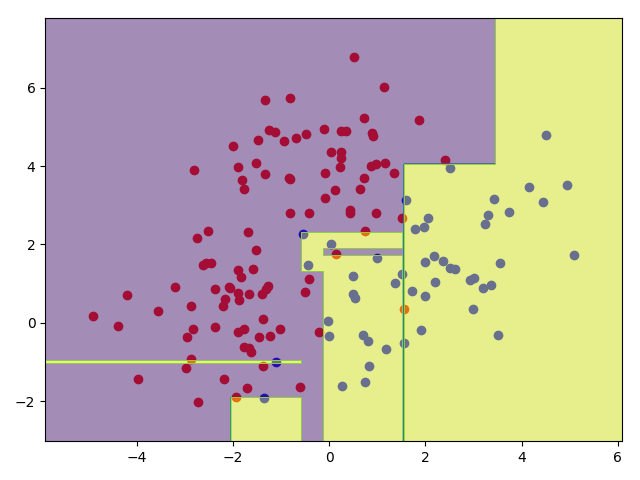
\includegraphics[width=.5\textwidth]{images/related_work/decision_tree_separator}
                    \caption[
                        Visualization of a decision tree separator trained over generated data in a two dimensional feature space.
                    ]{
                        \label{fig::decision_tree_separator}
                        Visualization of a decision tree separator trained over generated data in a two dimensional feature space.
                        The separator is composed exclusively of horizontal and vertical lines.
                        We can also see how the decision tree overfits by adding narrow splits to accomodate lone points surrounded by others with an opposite class.
                    }
                \end{figure}

                Up to now, we assumed the fact that the decision tree is already in place.
                The training step of this supervised classifier consists in determining its structure and all the thresholds.
                The goal is to have leafs with no prediction errors.
                In other words, all obsevations that end up in a leaf must be of the same class: the leaf is called pure.
                Consequently, to each node that is not pure would be associated a predicate that would hopefully distinguish amongst incoming observations.
                This is done recursively starting from the root.\\

                The choice of the splitting dimension and the threshold at each node is made in the aim of achieving the most gain in the ``purity'' of child nodes.
                As a consequence, there is a need of a metric $I$ that can describe the heterogenuity, as the opposite of purity, of a node.
                These are usually based on a probabilistic interpretation as they compute the fraction of observations $p_c$ that go through a node of class $c \in \left\{1, 2, \dots, C\right\}$.
                Three examples are provided:
                \begin{itemize}
                    \item Gini index:
                    \begin{equation}
                        \label{eq::gini}
                        I_G\left(\left(p_c\right)_{c=1, 2, \dots, C}\right) = \sum_{c=1}^{C} p_c \cdot \sum_{\substack{l=1, 2, \dots, C\\l \neq c}} p_l;
                    \end{equation}
                    \item Entropy:
                    \begin{equation}
                        \label{eq::entropy}
                        I_H\left(\left(p_c\right)_{c=1, 2, \dots, C}\right) = - \sum_{c=1}^{C} p_c \cdot \log_2(p_c);
                    \end{equation}
                    \item Variance:
                    \begin{equation}
                        \label{eq::variance_index}
                        I_V\left(\left(x_{d_s}^i\right)_{i\in S}\right) = \frac{1}{2 \cdot \vert S \vert^2} \cdot \sum_{(i,j) \in S\times S} \left(x_{d_s}^i - x_{d_s}^j\right),
                    \end{equation}
                    where:
                    \begin{conditions}
                        d_s & is the chosen dimension to split over;\\
                        S & $\subset \left\{1, 2, \dots, n\right\}$ is an set of indices.
                    \end{conditions}
                \end{itemize}
                Considering $S_b$ the set of indices of inputs going through a node $b$, one can compute the gain of a split at node $b$ as:
                \begin{equation}
                    \label{eq::split_gain}
                    G_b \triangleq I(S_b) - \sum_{c \in \left\{d_b(\bm{x}^i): i \in S_b\right\}} I(S_c)
                \end{equation}
                The optimal splitting dimension and threshold are chosen so that they maximizes the gain $G_b$.
                Details of how this is computed is outside ths scope of this manuscript and is not provided herein.
                For more information on the subject the reader may refer to the work of~\textcite{breiman1984classification}.\\

                Stopping only when total purity is achieved can yield complicated decision trees that overfit easily.
                This motivates the use for some early stopping criteria:
                \begin{itemize}
                    \item a minimal number of observations going through each node.
                    \item a minimal purity ratio computed as the ratio of all instances going through the node having the dominant class.
                    \item a maximal depth of the tree.
                \end{itemize}
                To conclude, the class at each leaf is taken as the dominant class of instances entering it.

            \paragraph{Bagging decision trees}
                \begin{figure}
                    \centering
                    \includestandalone[mode=buildnew, height=.4\textheight]{figures/random_forest/ensemble}
                    \caption[
                        Illustration of the principle of ensemble methods.
                    ]{
                        \label{fig::ensemble} Illustration of the principle of ensemble methods.
                        For each decision function $\forall l=1,2,3\;D_l$, is represented the set where the each classifier fails $F(D_l) \leftarrow \left\{(\bm{x}, y) \in \prod_{i=1}^{d}\mathscr{X}_i \times \left\{1,2,\dots,C\right\} : D_l(\bm{x}) \neq y\right\}$.
                        In the case of unweigthed bagging, the aggregated classifier will fail when more than half of the classifiers fail.
                        In this case, the set $F(D_{\text{bagging}})$ is the union of intersections of two different $F(D_l)$: $F(D_{\text{bagging}}) = \bigcup_{l\neq p} F(D_l) \cap F(D_p)$.
                        In this case where classifiers are diverse, the aggregated one fails less frequently than each single one.
                    }
                \end{figure}

                \begin{figure}
                    \centering
                    \ffigbox[\FBwidth]{
                        \begin{subfloatrow}[2]
                            \ffigbox[\FBwidth]{
                                \includestandalone[mode=buildnew, width=.45\textwidth]{figures/random_forest/circles_dt}
                            }{
                                \caption{
                                    \label{subfig::decision_tree_circles} Decision tree separator
                                }
                            }
                            \ffigbox[\FBwidth]{
                                \includestandalone[mode=buildnew, width=.45\textwidth]{figures/random_forest/circles_rf}
                            }{
                                \caption{
                                    \label{subfig::rf_circles} Random forest separator (in purple) with constituing decision trees
                                }
                            }
                        \end{subfloatrow}
                    }{
                        \caption[
                            Difference between a single decision tree and a random forest visualized in feature space for a generated toy data.
                        ]{
                            \label{fig::decision_tree_vs_rf}
                            Difference between a single decision tree and a random forest visualized in feature space for a generated toy data.
                            We see how a random forest aggregates multiple shallow decision trees in order to achieve a good generalization power instead of overfitting to the sampled data.
                        }
                    }
                \end{figure}

                While reducing the complexity of the decision tree can help avoid overfitting problems, one can risk, on the other hand, an underfitting in the classification.
                In order to find a compromise, an ensemble method can be adopted.
                The principle of this type of approaches is to multiply different underperforming classifiers and aggregate them together.
                These classifiers should be taken as diverse as possible in order to cover the whole feature space.
                The aggregation is achieved through a majority vote and, if the classifiers can provide probabilities, the vote can be weighted by the latter.
                This is illustrated in Figure~\ref{fig::ensemble}.
                Formally, the decision function of an unweighted aggregation of classifiers $\left(D_l\right)_{l=1,2,\dots,L}$ can be written as:
                \begin{equation}
                    \label{eq::decision_function_hard_ensemble}
                    \begin{aligned}
                        D_{\text{hard ensemble}, \left(D_l\right)_{l=1,2,\dots,L}}: \prod_{i=1}^{d}\mathscr{X}_i &\rightarrow \left\{1,2,\dots,C\right\}\\
                        \bm{x} &\mapsto \arg \max_{c=1,2,\dots,C}\lvert\left\{l\in\left\{1,2,\dots,L\right\}: D_l(\bm{x}) = c\right\}\rvert
                    \end{aligned},
                \end{equation}
                while the weighted aggregation using classifier output probabilities $\left(p_l\right)_{l=1,2,\dots,L}$ is expressed as:
                \begin{equation}
                    \label{eq::decision_function_weighted_ensemble}
                    \begin{aligned}
                        D_{\text{weighted ensemble}, \left((D_l, p_l)\right)_{l=1,2,\dots,L}}: \prod_{i=1}^{d}\mathscr{X}_i &\rightarrow \left\{1,2,\dots,C\right\}\\
                        \bm{x} &\mapsto \arg \max_{c=1,2,\dots,C} \sum_{l=1}^{L} p_l\left(D_l(\bm{x}) = c\right) 
                    \end{aligned}.
                \end{equation}

                Bagging is an instance of ensemble approach.
                In order to have different classifiers specializing in a certain pattern, each one is trained on a randomly determined subset of the training data~\parencite{breiman1996bagging}.
                The idea is that each one of these subsets would exhibit a particular aspect that is crucial for the classification.
                The aggregation of each classifier knowledge would eventually help generalize in prediction time.\\

                Random forest do not only rely on a simple bagging but also on a second random sampling: this time it is on the dimensions.
                When splitting a node at training time, only a subset of randomly chosen dimensions is considered~\parencite{breiman2001random}.
                We depict in Figure~\ref{fig::decision_tree_vs_rf} the difference between a random forest and a single decision tree.

            \paragraph{Properties}
                Random forests are often used in practice as they offer some advantages.
                Hereafter are listed some of these:
                \begin{itemize}
                    \item As decision trees deal with each feature independently, they can natively, as well as Random Forests, handle heterogenous data.
                        It can handle boolean features along with integer or real ones.
                    \item Since at each time only a subset of features are considered, Random Forests can scale easily under high dimensionality.
                    \item The ensemble character of Random Forests allows them to adapt to outliers and hence have a good generalization power.
                    \item Prediction relies on simple comparisons and can be computed quickly.
                    \item They inherently yield probabilisties that are consistent.
                \end{itemize}
                As seen with \glspl{acr::svm}, Random Forests have also some issues:
                \begin{itemize}
                    \item It is not simple to interpret results of Random Forests and connect specific trees to recongnizable patterns.
                    \item They can take up a lot of memory to store all trees.
                            They can also require a lot of computations to train.
                    \item They do not allow the possibility of using kernels to represent the data.
                    \item They does not handle well imbalanced datasets and must be adapted accordingly.
                \end{itemize}
                
    \subsection{\textsc{Feature extraction}}
        \label{subsec::state_of_the_art::mlpr::feature_extraction}
            Before feeding observations to classifiers, representative features are extracted.
            These are usually vectors from a finite dimensional space called feature space.
            In the previous subsection, we considered a special case of feature spaces $\mathbb{R}^d$.\\

            Feature extraction is not straight-forward.
            It is either hand crafted or learned (using deep learning) to fit a specific need.
            Image feature extraction is one such example where attributes are drawn from images in order to describe specific patterns such as edges~\parencite{canny1986computational}, corners~\parencite{harris1988combined} or \gls{acr::sift}~\parencite{lowe2004distinctive}.
            Herein, we present a specific type of feature extractors called \glspl{acr::scatnet}.
            Images can also be considered as specific type of graphs with a grid structure.
            In the same sense, features can be extracted from graphs.
            We will describe hence how to describe graphs for classification.

        \subsubsection{\textsc{\acrlong*{acr::scatnet} for image classification}}
            \glspl{acr::scatnet} can be seen as a reverse engineered convolutional network.
            They are built mainly relying on wavelet filters which are used to imitate filters from \glspl{acr::cnn}.
            The latter learns automatically an image representation $\Phi$ trying to minimize a learning loss function.
            \Glspl{acr::scatnet}, on the other hand, make use of mathematical properties of the image signal.\\

            Some propeties are always required in order to acheive a good representation $\Phi$ of an image. 
            A scene that is captured from different point of views, while yielding different images, should have close representations.
            Just as with interset point detection~\parencite{harris1988combined,lowe2004distinctive}, the representation of an image should be invariant to scale, translation and rotation~\parencite{mallat2012group,sifre2013rotation,bruna2013invariant}.
            Since images illustrate not only rigid objects, a good representation should allow small local deformations in the signal that can be attributed to distortions of non-rigid objects.\\

            \paragraph{Mathematical notations}
                To formalize these properties, we introduce some mathematical notations.
                \subparagraph{Action of a group}
                    Let $x: u \mapsto x(u)$ be an image (or any signal in general) and $(G, *)$ a group such as the set of translation operators on signals.
                    The action of $g\in G$ on $x$ is written as:
                    \begin{equation}
                        \label{eq::action_group}
                        L_g(x): u \mapsto x\left(g^{-1}(u)\right).
                    \end{equation}
                
                    As an example, we can study the case of $T_{\mathbb{R}^2}$ a translation group on $\mathbb{R}^2$.
                    This group is isomorphic to $\mathbb{R}^2$: \textit{i.e.} $(T_{\mathbb{R}^2}, \circ) \cong (\mathbb{R}^2, +)$.
                    Let $v$ be a vector in $\mathbb{R}^2$.
                    We denote a translation by vector $v$ by $t_v: u \mapsto u + v$.
                    Its inverse verifies $t_v^{-1} = t_{-v}$.
                    For $v \in \mathbb{R}^2$, we can express the translation applied to signal as:
                    \begin{equation}
                        \label{eq::action_translation}
                        L_{t_v}(x): u \mapsto x\left(u - v\right).
                    \end{equation}
                    Equally, if we consider the rotation group $SO(2)$ which is isomorphic to the unit circle, and write a rotation of angle $\theta \in [0, 2\cdot\pi)$ as $r_{\theta}$, we express the action of that group as:
                    \begin{equation}
                        \label{eq::action_rotation}
                        L_{r_{\theta}}(x): u \mapsto x\left(r_{-\theta}(u)\right).
                    \end{equation}
                    Rotations and translations are not commutative in the general case.
                    This justifies the definition of a roto-translation group, called also the rigid motion group and denoted $SE(2)$.
                    Such a group is isomorphic to $\mathbb{R}^2 \times SO(2)$.
                    Let $v \in \mathbb{R}^2$ and $\theta \in [0, 2\cdot\pi)$, a member of such a group is defined as:
                    \begin{equation}
                        \label{eq::roto-translation}
                        g_{\theta, v} \triangleq t_v \circ r_{\theta} = r_{\theta} \circ t_{r_{-\theta}(v)}
                    \end{equation}
                    and its inverse is expressed then as $g_{\theta, v}^{-1} = r_{-\theta} \circ t_{-v}$.
                    Hence we can write:
                    \begin{equation}
                        \label{eq::action_roto-translation}
                        L_{g_{\theta, v}}(x): u \mapsto x \left(r_{-\theta}(u - v)\right).
                    \end{equation}
                
                \subparagraph{Group convolution}
                    A convolution over a locally compact topological group $G$ is defined as:
                    \begin{equation}
                        \label{eq::group_signal_convolution}
                        x \ostar y: u \mapsto \int_{h\in G} x(h)\cdot y(h^{-1}(u)) \cdot dh
                    \end{equation}
                    where:
                    \begin{conditions}
                        dh & is the Haar measure on $G$.
                    \end{conditions}

                    For signals $x$ and $y$ that take inputs on the plane $\mathbb{R}^2$, we can recognize the usual definition of a convolution:
                    \begin{equation}
                        \label{eq::translation_convolution}
                        x \star y: u \mapsto \int_{v \in \mathbb{R}^2} x(v)\cdot y(u - v) \cdot dv
                    \end{equation}

                    Applied in the roto-translation case to signals $x(u, \theta)$ on pairs from $\mathbb{R}^2 \times [0, 2\cdot\pi)$, we write:
                    \begin{equation}
                        \label{eq::roto-translation_convolution}
                        x \ostar_{SE(2)} y: (u, \theta) \mapsto \int_{\substack{v \in \mathbb{R}^2\\\omega \in [0, 2\cdot\pi)}} x(v, \omega)\cdot y(r_{-\omega}(u - v), \theta - \omega) \cdot dv d\omega
                    \end{equation}
            
            \paragraph{Invariance: formulation}
                $\Phi$ is said to be invariant to $g$ if and only if:
                \begin{equation}
                    \label{eq::invariance}
                    \Phi\circ L_g\left(x\right) = \Phi(x),
                \end{equation}
                and covariant if and only if:
                \begin{equation}
                    \label{eq::covariance}
                    \Phi\circ L_g\left(x\right) = L_g\circ\Phi(x).
                \end{equation}
                Images of similar objects should have a representations that are also similar.
                Using Euclidean distances as a similarity measure, this property implies $\Phi$ to be contractive~\parencite{bruna2013invariant}.
                Given two images $x$ and $y$, we write:
                \begin{equation}
                    \label{eq::contractive}
                    \Vert \Phi(x) - \Phi(y) \Vert \leq \Vert x-y \Vert.
                \end{equation}
                The mapping $\Phi$ should be stable under small local deformations.
                A local deformation is modeled as a diffeomorphism\footnote{A differentiable bijection which inverse is differentiable also.} $\tau$.
                A small one is formalized as a diffeomorphism $\tau$ that verifies $\Vert\nabla \tau\Vert_\infty < 1$~\parencite{bruna2013invariant,sifre2013rotation,mallat2012group}.
                A good transform $\Phi$ , there exists a constant $C>0$ such that for any image $x$:
                \begin{equation}
                    \label{eq::stable_deformation}
                    \exists C >0, \forall x \in \mathscr{I}\quad \Vert \Phi(x) - \Phi\circ L_\tau(x) \Vert \leq C \cdot \Vert x\Vert \cdot \Vert\nabla \tau\Vert_\infty.
                \end{equation}
                where:
                \begin{conditions}
                    \mathscr{I} & is the set of all possible signals;\\
                    L_\tau(x) & $u \mapsto x(u - \tau(u))$ is the action of the deformation $tau$ on a signal $x$.
                \end{conditions}
                We say that $Phi$ is Lipschitz stable to deformations.

            \paragraph{\gls*{acr::scatnet}: a reverse engineered \gls*{acr::cnn}}
                \glspl{acr::cnn} learn such a representation which verifies these previous conditions stated in Equations~\ref{eq::contractive},~\ref{eq::invariance} and~\ref{eq::stable_deformation}.
                In fact, it is possible by virtue of some basic building blocs.
                First, since the weights are learned based on a classification objetive, images with similar content are supposed to be mapped to the same region.
                Second, pooling layers in \glspl{acr::cnn} provide a solution for invariance to translations and local deformations up to a scale.\\

                The \gls{acr::scatnet} being a reverse engineered \gls{acr::cnn}, formalizes these ideas using wavelet transforms.
                The idea is to apply linear convolutional operators followed by a non-linearity and some pooling operators.
                In a \gls{acr::scatnet} the learned filters are replaced by a specific wavelet decomposition, the non-linearity is acheived using the modulus operator and pooling is obtained through a low pass filter.
                The low-pass filter is critical for the invariance condition, while the lost high frequencies are retrieved using the wavelet convolutions.
                The non-linearity, just as in \glspl{acr::cnn}, is necessary in order to obtain interesting non-linear final representations.\\

                \subparagraph{Wavelets filter bank}
                    We need two sets of wavelets: spatial and angular.
                    Spatial wavelet filters are derived based on a mother wavelet $\psi: \mathbb{R}^2 \rightarrow \mathbb{C}$ as follows:
                    \begin{equation}
                        \label{eq::translation_filter_bank}
                        \psi_{i,\theta} : u\mapsto 2^{-2\cdot i}\cdot\psi\left(2^{-i}\cdot r_{-\theta}(u)\right).
                    \end{equation}
                    We also need a low-pass averaging filter $\phi: \mathbb{R}^2 \rightarrow \mathbb{R}$ scaled up to a desired size:
                    \begin{equation}
                        \label{eq::translation_low_pass}
                        \phi_I: u\mapsto 2^{-2\cdot I}\cdot\phi\left(2^{-I}\cdot u\right)
                    \end{equation}
                    The angular wavelets are computed using $2\cdot\pi$-periodic mother wavelet $\bar\psi: \mathbb{R}^2 \rightarrow \mathbb{C}$ scaled as follows:
                    \begin{equation}
                        \label{eq::angular_filter_bank}
                        \bar\psi_{\iota}: \omega \mapsto 2^{-\iota}\cdot\bar\psi\left(2^{-i}\cdot \omega\right)
                    \end{equation}
                    We also define need the constant averaging filter\footnote{It corresponds to a zero scale filter} defined as:
                    \begin{equation}
                        \label{eq::angular_low_pass}
                        \bar\phi: \theta \mapsto \frac{1}{2\cdot\pi}
                    \end{equation}
                    Based on the spatial filter bank defined in Equation~\ref{eq::translation_filter_bank} and the angular one from Equation~\ref{eq::angular_filter_bank}, we define rigid motion wavelets in the next equations:
                    \begin{align}
                        \label{eq::roto-translation_filter_bank}
                        \forall i\neq I, \theta \neq 0, \iota \neq 0 \quad \tilde{\psi}_{i, \theta, \iota}(u, \omega) &= \psi_{i,\theta}(u) \cdot \bar\psi_{\iota}(\omega)\\
                        \forall \iota \neq 0 \quad \tilde{\psi}_{I, 0, \iota}(u, \omega) &= \phi_I(u) \cdot \bar\psi_{\iota}(\omega)\\
                        \forall i\neq I, \theta \neq 0 \quad \tilde{\psi}_{i, \theta, 0}(u, \omega) &= \psi_{i,\theta}(u) \cdot \bar\phi(\omega).
                    \end{align}
                    The corresponding rigid motion averaging filter is obtained as:
                    \begin{align}
                        \label{eq::roto-translation_low_pass}
                        \tilde{\phi}(u, \omega) &= \tilde{\psi}_{I, 0, 0}(u, \omega) = \phi_I(u) \cdot \bar\phi(\omega) \nonumber \\
                        \tilde{\phi}(u, \omega) &= \frac{1}{2\cdot\pi} \cdot \phi_I(u)
                    \end{align}
                    These are separable filters that can help speed up the convolution computations as shown in~\textcite{sifre2013rotation}.
                    In practice, $\psi$(\textit{resp.} $\bar\psi$) are taken as two (\textit{resp.} one) dimensional Morlet wavelets (\textit{cf.} Subfigure~\ref{subfig::morlet_filters}), while $\phi$ is taken as a Guassian~\parencite{oyallon2015deep,sifre2013rotation,bruna2013invariant}.
                    A finite number $L$ of orientations are possible for angle indices: $\theta \in \left\{\frac{l\cdot\pi}{L}: l=1,2\dots,L\right\}$.
                    In Figure~\ref{fig::morlet_vs_learned}, we can see that how the defined filter bank is similar to the ones learned by a \gls{acr::cnn}.
                    \begin{figure}
                        \centering
                        \ffigbox{
                            \ffigbox[\FBwidth]{
                                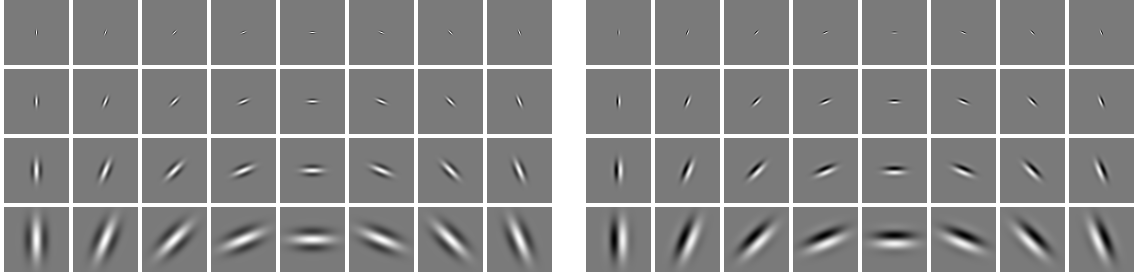
\includegraphics[width=\textwidth]{images/related_work/morlet_wavelets}
                            }{
                                \label{subfig::morlet_filters}
                                \caption[
                                    Morlet wavelets at different scales ($I=5$) and orientations ($L=8$).
                                ]{
                                    Morlet wavelets at different scales ($I=5$) and orientations ($L=8$).
                                    Left are presented the real part while the imaginary part is on the right.
                                    Image taken from~\parencite{sifre2013rotation}.
                                }
                            }
                            \ffigbox[\FBwidth]{
                                \begin{tabular}{@{}c@{}}
                                    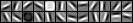
\includegraphics[width=.5\textwidth]{images/related_work/first_layer_cnn}\\
                                    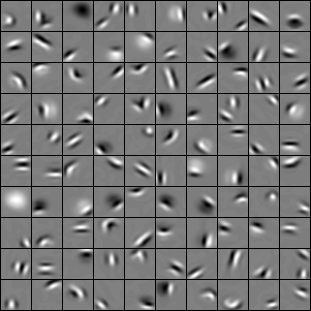
\includegraphics[width=.75\textwidth]{images/related_work/second_layer_cnn}
                                \end{tabular}
                            }{
                                \label{subfig::learned_filters}
                                \caption[
                                    Learned filters at the first and second layers of a \acrshort*{acr::cnn}.
                                ]{
                                    Learned filters at the first (top) and second (bottom) layers of a \gls{acr::cnn}.
                                    Image taken from~\parencite{lee2009convolutional}.
                                }
                            }
                        }{
                            \caption[
                                Comparison of the Morlet wavelet bank and the first and second layer filters learned from a \acrshort*{acr::cnn}.
                            ]{
                                \label{fig::morlet_vs_learned}
                                Comparison of the Morlet wavelet bank and the first and second layer filters learned from a \gls{acr::cnn}.
                                The latter can be distinguished into two classes:
                                an averaging filter that could be likened to $\phi$ and rotated and scaled (only in the second layer) filters that looks like Morlet wavelets.
                            }
                        }
                    \end{figure}
                     
                \subparagraph{The wavelet-modulus operator}
                    A wavelet transform of a signal $x$ consists in representing it using a wavelet filter bank: $\left(x\ostar\psi_{\lambda}\right)_{\lambda}$.
                    Depending on the transformed signals, two versions of wavelet transforms are possible.
                    If the signal takes one variable $u in \mathbb{R}^2$ then we write:
                    \begin{equation}
                        \label{eq::wavelet_transform_1}
                        W: x \mapsto \left(x\star\psi_{i, \theta}\right)_{\substack{i=1, 2 \dots, I \\ \theta \in \left\{\frac{l\cdot\pi}{L}: l=1,2\dots,L\right\}}},
                    \end{equation}
                    if it takes two variables $(u, \omega) \in \mathbb{R}^2 \times [0, 2\cdot\pi)$ it becomes:
                    \begin{equation}
                        \label{eq::wavelet_transform_2}
                        \widetilde{W}: x \mapsto \left(x\ostar_{SE(2)}\psi_{i, \theta, \iota}\right)_{\substack{i=1, 2 \dots, I \\ \theta \in \left\{\frac{l\cdot\pi}{L}: l=1,2\dots,L\right\}\\\iota=1,2\dots,\lfloor\log_2(L)\rfloor}}.
                    \end{equation}
                    An image is a discretization of a two dimensional signal.
                    As a consequence, we can only apply the first transform in Equation~\ref{eq::wavelet_transform_1}.
                    The result of such a mapping is an example of a signal on wich one can apply the second transform from Equation~\ref{eq::wavelet_transform_2}.
                    For the right choice of wavelets, these operators can be proven to be invertible, contractive and Lipschitz stable to deformations~\parencite{mallat2012group}.\\

                    By applying a modulus we get the basic building bloc of \glspl{acr::scatnet} called the wavelet-modulus operator: $x \mapsto \vert x\ostar\psi_{\lambda} \vert$.
                    This is delineated for the two cases as follows:
                    \begin{align}
                        \label{eq::wavelet-modulus_1_2}
                        U_{i, \theta}: x &\mapsto \vert x\star\psi_{i, \theta}\vert\\
                        \widetilde{U}_{i, \theta, \iota}: x &\mapsto \vert x\ostar_{SE(2)}\psi_{i, \theta, \iota} \vert
                    \end{align}
                    These operators are proven to be covariant to translations and rotations~\parencite{mallat2012group,sifre2013rotation}: \textit{i.e.} for a couple $(v, \vartheta) \in \mathbb{R}^2 \times [0, 2\cdot\pi)$:
                    \begin{align}
                        \label{eq::covariance_wavelet-modulus}
                        L_{g_{v, \vartheta}} \circ U_{i, \theta} &= U_{i, \theta} \circ L_{g_{v, \vartheta}}\\
                        L_{g_{v, \vartheta}} \circ \widetilde{U}_{i, \theta, \iota} &= U_{i, \theta, \iota} \circ L_{g_{v, \vartheta}}.
                    \end{align}
                    These conditions may remind the reader of the work of~\textcite{cohen2016group} on \gls{acr::gcnn}.
                
                \subparagraph{The average pooling}
                    Contrarily to~\parencite{cohen2016group}, the pooling operations differ.
                    \glspl{acr::gcnn} rely on max-pooling as standard practice in \glspl{acr::cnn}.
                    This operator is actually covariant to actions of the rigid movement group.
                    \parencite{bruna2013invariant, sifre2013rotation,oyallon2015deep}, however, rely on averaging (or low-pass) filters as pooling operators.

                    Considering the rigid mouvement as a nuisance,~\parencite{sifre2013rotation} considers invariance with regards to the roto-translation group.
                    To do so they filter any signal $x(u)$ using $\phi_I$ yielding a signal:
                    \begin{equation}
                        \label{eq::pool_bi-dim}
                        P_I: x \mapsto x \star \phi_I (u).
                    \end{equation}
                    For signals $\tilde{x}(u, omega)$ they are averaged using $\tilde{\phi}_I$ and giving as ouput:
                    \begin{equation}
                        \label{eq::pool_bi-dim-angular}
                        \widetilde{P}_I: x \mapsto \tilde{x} \ostar_{SE(2)} \tilde{\phi}_I (u, \omega).
                    \end{equation}

                    These operators are actually invariant to translation and rotation:
                    \begin{align}
                        \label{eq::invariance_pooling}
                        P_I = P_I \circ L_{t_v}\\
                        \tilde{P}_I = \tilde{P}_I \circ L_{g_{v, \vartheta}}.
                    \end{align}

                \subparagraph{Scattering coefficients}
                    Applying the first operation~\ref{eq::pool_bi-dim} to the input image defines the first scattering coefficient:
                    \begin{equation}
                        \label{eq::scatter_input}
                        S_0[x](u) \triangleq x \star \phi_I (u).
                    \end{equation}
                    
                    To the image, is applied the wavelet-modulus operator giving coefficients $U_{i_1, \theta_1}(x)$.
                    The latter is averaged using the second operation~\ref{eq::pool_bi-dim-angular}.
                    This defines the second layer of scattering coefficients:
                    \begin{equation}
                        \label{eq::scatter_first}
                        S_1[x](u, i_1, \theta_1) \triangleq U_{i_1, \bullet} \ostar_{SE(2)} \tilde{\phi}_I(u, \theta_1).
                    \end{equation}

                    At the second level is applied the wavelet-modulus operator retrieves the high-frequencies lost after the low-pass filter using yet another time the wavelet-modulus operator yielding:
                    \begin{equation}
                        \label{eq::cascade_second}
                        \widetilde{U}_{i_2,\iota_2, \theta_2} \circ U_{i_1, \theta_1}(x)
                    \end{equation}
                    Once again, an average pooling is applied on the latter:
                    \begin{equation}
                        \label{eq::scatter_second}
                        S_2[x](u, i_1, \theta_1, i_2, \theta_2, \iota_2) \triangleq \widetilde{U}_{i_2,\iota_2, \theta_2} \circ U_{i_1, \bullet} \ostar_{SE(2)} \tilde{\phi}_I(u, \theta_1).
                    \end{equation}
                    
                    This can be reapplied further giving casacaded scattering coefficients at level $m$:
                    \begin{equation}
                        \label{eq::scatter_second}
                        S_m[x](u, p) \triangleq \widetilde{U}_{\lambda_m} \circ \widetilde{U}_{\lambda_{m-1}} \dots \circ \widetilde{U}_{\lambda_2} \circ U_{i_1, \bullet} \ostar_{SE(2)} \tilde{\phi}_I(u, \theta_1).
                    \end{equation}
                    where:
                    \begin{conditions}
                        p & $i_1, \theta_1, \lambda_2 \dots, \lambda_{m-1}, \lambda_m$ and is called a path;\\
                        \lambda_k & $i_k, \theta_k, \iota_k$.
                    \end{conditions}

                    The scattering coefficients are proved to be contractive and Lipschitz stable to deformations~\parencite{mallat2012group}.
                    Moreover, they are invariant to actions of the group of rigid movement.
                    In fact, concatenating a covariant operator and an invariant one yields an invariant operator~\parencite{mallat2012group,sifre2013rotation}.

                    The energy of the signal is concentrated along increasing scale paths: \textit{i.e.} $\forall k=1,2,\dots,m-1 \; i_{k+1} > i_k$.
                    This implies that computing coefficients along these paths is sufficient~\parencite{bruna2013invariant,sifre2013rotation,oyallon2015deep}.
                    Furthermore, only the first two layers are computed as they concentrate most the energy of the signal~\parencite{bruna2013invariant,sifre2013rotation,oyallon2015deep}.
                    This yields an efficient way of computing a scattering transform as discussed by~\textcite{oyallon2015deep,sifre2013rotation}.\\

                    \textcite{sifre2013rotation} goes on to propose a way to make the scattering invariant to scale effects also.
                    This is done by introducing a logarithm that linearizes the dependency of scattering coefficients to scales $i_1$ and $i_2$~\parencite{sifre2013rotation,oyallon2015deep}.
                    An scale-space averaging is thus applied to achieve the sought invariance.\\

                    In contrast,~\textcite{oyallon2015deep} proposes to keep only the translation invariance and let the classifier decide on the relevance of rotation and scale invariance, much like in~\parencite{cohen2016group}.
                    To do so only a spatial averaging convoluation is applied as $x \mapsto \tilde{x}(\bullet, \omega) \star \phi_I$ which is covariant to rotations.
                    Similarly, they drop the scale-space averaging at the end, while the logarithm guaranties the covariance of the signal to scaling effects.
                    The operations are also conducted in a way that renders the shape of the \gls{acr::scatnet}, shown in Figure~\ref{fig::scatnet}, more like that of \gls{acr::cnn}.

                    \begin{figure}
                        \centering
                        \includestandalone[mode=buildnew, width=\textwidth]{figures/scattering_network}
                        \caption[
                            Illustration of a \acrshort*{acr::scatnet}.
                        ]{
                            \label{fig::scatnet} Illustration of a \gls{acr::scatnet}.
                            At each level are computed are computed convolutions with a filter bank followed by a modulus operator.
                            The scattering coefficients are obtained then by a low-pass filter (in blue).
                            In practice, scattering coefficients are only computed for increasing scale paths up to level $2$.
                        }
                    \end{figure}

        \subsubsection{\textsc{Kernels for graph classification}}
            \label{subsec::state_of_the_art::mlpr::graph_classification}
            Standard machine learning practice usually assumes that the observed instances live in a finite dimensional space.
            This is not always the case.
            In fact, graphs can have varying numbers of nodes and edges.
            Moreover, they can be different while providing the same structural information: we say they are isomorphic.
            A valid representation for graphs should then take care of these two issues: incorporate all possible graph sizes and be invariant to graph isomorphisms.
            As accustomed in statistical learning, one way to alleviate these issues is to directly compare graphs using kernels as seen previously in sub-subsection~\ref{subsubsec::state_of_the_art::mlpr::classifiers::svm}.\\
            
            This sub-subsection does not aim at presenting a thourough survey of graph kernels.
            The work of~\textcite{ghosh2018journey} categorizes graph kernels depending on the used methodology.
            A different approach is proposed in~\textcite{kriege2019survey}, where they study graph kernels based on the underlying graphs.\\

            Apart from the structure of the graph, kernels should also take into account the labels or continuous attributes assigned to a graph.
            These could be given at node level or edge level.
            We will present hereafter some graph kernels which were used in this work, namely, continuously node attributed ones, as well as those devoted only to its structural properties.\\

            \paragraph{Basic kernels}
                Let $G = \left(V, E\right)$ an undirected graph with vertices $v\in V$ and edges $e \in E =\left\{\left\{u, v\right\}: (u, v) \in V\times V\right\}$.
                We can give attributes to each node $a: V \rightarrow \mathbb{R}^{d_V}$ or edges $b: E \rightarrow \mathbb{R}^{d_E}$.\\

                The most basic graph kernel would correspond to a scalar product of a global hashing vector of all attributes.
                This is possible through the use of a histogram function for instance.
                This type of functions is described in details in Subsection~\ref{subsec::learned_evaluation::baseline::geometric}.\\

                Let $S\left(G, a(\bullet)_i\right): \mathbb{R}^{\vert V\vert} \rightarrow \mathbb{R}^{l_i}$ (\textit{resp.} $S\left(G, b(\bullet)_i\right): \mathbb{R}^{\vert E\vert} \rightarrow \mathbb{R}^{m_i}$) be a hashing function that describes the distribution of attributes $i$ of all nodes (\textit{resp.} edges) of graph $G$ as a $\mathbb{R}^{l_i}$ (\textit{resp.} $\mathbb{R}^{m_i}$) vector.
                We can build a node based feature vector for the graph $G$:
                \begin{equation}
                    \label{eq::feature_node_graph}
                    \Phi_V(G) \triangleq \begin{bmatrix}
                        S\left(G, a(\bullet)_1\right)\\
                        S\left(G, a(\bullet)_2\right)\\
                        \vdots\\
                        S\left(G, a(\bullet)_{d_V}\right)
                    \end{bmatrix} \in \mathbb{R}^{\sum_{i=1}^{d_V} l_i}
                \end{equation}
                and an edge based one:
                \begin{equation}
                    \label{eq::feature_node_graph}
                    \Phi_E(G) \triangleq \begin{bmatrix}
                        S\left(G, b(\bullet)_1\right)\\
                        S\left(G, b(\bullet)_2\right)\\
                        \vdots\\
                        S\left(G, b(\bullet)_{d_E}\right)
                    \end{bmatrix} \in \mathbb{R}^{\sum_{i=1}^{d_E} m_i}.
                \end{equation}

                Based on a base kernel on vectors $\kappa$ (\textit{cf.} sub-subsection~\ref{subsubsec::state_of_the_art::mlpr::classifiers::svm}), we can compute the similarity between two graphs $G = \left(V, E\right)$ and $G' = \left(V', E'\right)$:
                \begin{align}
                    \label{eq::feature_graph_kernel_nodes}
                    k_V(G, G') &\triangleq \kappa(\Phi_V(G), \Phi_V(G'))\\
                    \label{eq::feature_graph_kernel_edges}
                    k_E(G, G') &\triangleq \kappa(\Phi_E(G), \Phi_E(G')).
                \end{align}
                Concatenating both feature vectors would amount to a simple addition of these kernels:
                \begin{equation}
                    \label{eq::feature_graph_kernel_sum}
                    k(G, G') \triangleq k_V(G, G') + k_E(G, G').
                \end{equation}

                This type of kernels is versatile as it can be applied to node and edge attributes as well as labels (with the right choice of hashing function).
                However, it does not take into account the structure of the graph.
                It is mainly used as a baseline for graph feature extraction.
                The work of~\textcite{shervashidze2011weisfeiler} is an example of kernels that uses the same idea to describe graphs while taking account of their structure.
            
            \paragraph{Random walk kernel}
                In order to define this kernel, we need to defined the adjacency matrix $A$ of a graph $G$:
                \begin{equation}
                    \label{eq::adjacency_matrix}
                    A \triangleq \left(\delta_{\left\{u,v\right\}\in E}\right)_{(u, v) \in V\times V}
                \end{equation}
                and the diagonal matrix of node degrees $D\triangleq \operatorname{diag}\left(\sum_{v \in V}A_{uv}\right)_{u \in V}$.
                We also denote the normalized adjacency matrix as:
                \begin{equation}
                    \label{eq::normalized_adjacency_matrix}
                    P \triangleq A\cdot D^{-1}
                \end{equation}

                The latter could be interpreted as a transition probability matrix of a random walk on the graph:
                $P_{uv}$ is the probability of choosing $u$ as the next node to visit starting from $v$.
                Similarly, $\left(P^k\right)_{uv}$ expresses the probability of being in node $u$ after $k$ iterations, starting from $v$.
                A random walk starts with an initial distribution $p$ over the nodes.
                After $k$ iterations, the distribution is $P^k\cdot p$.
                At any time, the walk can end with a probability $q_u$ at node $u$.
                $p$ and $q$ are used to encode prior information of the graph~\parencite{vishwanathan2010graph}.\\
                
                \subparagraph{Simultaneous random walk}
                    To compare two graphs \(G\) and \(G'\) using random walks, we start by defining the direct product graph $G_{\times} = \left(V_{\times}, E_{\times}\right)$ where:
                    \begin{align}
                        \label{eq::direct_product_graph}
                        V_{\times} &\triangleq V \times V'\\
                        E_{\times} &\triangleq \left\{\left\{(u, u'), (v, v')\right\}: \left\{u,v\right\} \in E \wedge \left\{u',v'\right\} \in E'\right\}.
                    \end{align}
                    This is vizualized in Figure~\ref{fig::direct_product_graph}.
                    \begin{figure}[htbp]
                        \centering
                        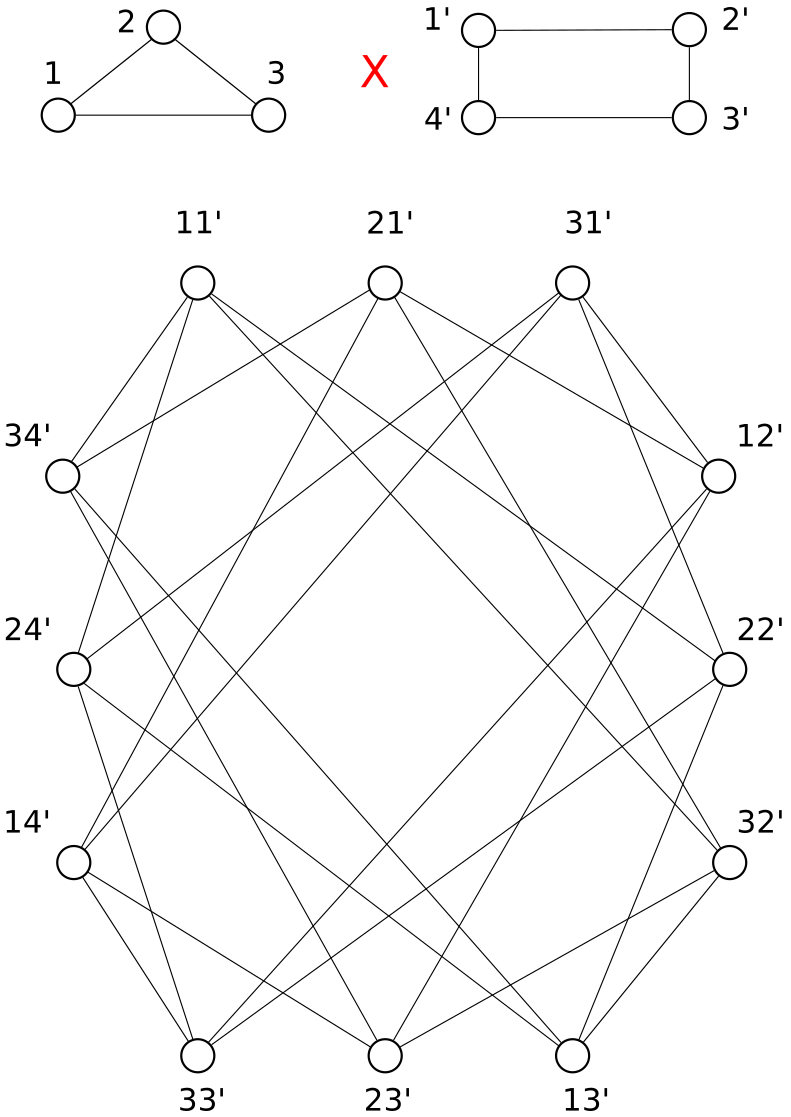
\includegraphics[height=.4\textheight]{images/related_work/direct_product_graphs}
                        \caption[
                            Depiction of a direct product of two graphs.
                        ]{
                            \label{fig::direct_product_graph}
                            Depiction of a direct product (bottom) of two graphs (top).
                            Nodes adjacent in $G_{\times}$ correspond to adjacent nodes in both graphs.
                            Image taken from~\parencite{vishwanathan2010graph}.
                        }
                    \end{figure}

                    For the direct product graph, we compute adjacency matrices, initial probability distribution and stopping probabilities as follows:
                    \begin{align}
                        \label{eq::direct_product_graph_walk}
                        A_{\times} &= A \otimes A'\\
                        P_{\times} &= P \otimes P'\\
                        p_{\times} &= p \otimes p'\\
                        q_{\times} &= q \otimes q'
                    \end{align}
                    where:
                    \begin{conditions}
                        \otimes & referes to the Kronecker product.
                    \end{conditions}
                    In fact, a random walk on $G_{\times}$ is equivalent to a simultaneous random walk on $G$ and $G'$~\parencite{hammack2011handbook}.\\

                    A random walk on a graph depends heavily on the its structure.
                    In consequence, a random walk on the direct product graph can be used as an indicator of the similarity in structure of both graphs $G$ and $G'$.
                    It is defined as:
                    \begin{equation}
                        \label{eq::random_walk_kernel}
                        k_{rw}(G, G') \triangleq \sum_{k=0}^\infty \lambda_k \cdot q_{\times}^T\cdot P_{\times}\cdot p_{\times}.
                    \end{equation}

                \subparagraph{Special cases}
                    This defintion actually generalizes a family of graph kernels based on walks on graphs~\parencite{vishwanathan2010graph}.
                    The choice of the series $\left(\lambda_k\right)_{k\in \mathbb{N}}$ is critical, as the kernel defined in Equation~\ref{eq::random_walk_kernel} can diverge.
                    It is taken to be non-negative in order in ensure the positive semi-definite of the kernel.\\

                    Setting $p_{\times} \propto 1$ and $q_{\times} \propto 1$ and , two special cases are of interest.
                    \begin{itemize}
                        \item $\forall k\in \mathbb{N} \; \lambda_k = \lambda^k$: this gives rise to a geometric random kernel:
                                \begin{equation}
                                    \label{eq::geometric_random_kernel}
                                    k_{grw}(G, G') = \begin{bmatrix}
                                        1, 1\dots,1
                                    \end{bmatrix}\cdot \left(I - \lambda\cdot A_{\times}\right)^{-1}\cdot\begin{bmatrix}
                                        1\\
                                        1\\
                                        \vdots\\
                                        1
                                    \end{bmatrix}.
                                \end{equation}
                                For this kernel to be valid, $\lambda$ should be less than the largest eigenvalue of $A_{\times}$.
                        \item $\forall k\in \mathbb{N} \; \lambda_k = \frac{\lambda^k}{k!}$: this yields the so called exponential random kernel:
                                \begin{equation}
                                    \label{eq::geometric_random_kernel}
                                    k_{erw}(G, G') = \begin{bmatrix}
                                        1, 1\dots,1
                                    \end{bmatrix}\cdot \exp\left(\lambda\cdot A_{\times}\right)\cdot\begin{bmatrix}
                                        1\\
                                        1\\
                                        \vdots\\
                                        1
                                    \end{bmatrix}.
                                \end{equation}
                    \end{itemize}
                    These graph kernels where already defined in~\parencite{gartner2003graph}.\\

                Computationally, these involve heavy computations.
                \textcite{vishwanathan2010graph} proposed efficient numerical algorithms to aleviate this problem.
                However, these graphs suffer from other issues.
                First, the kernel does take into account the attributes of graphs of they exist, although it is possible to adapt.
                Second, these graphs suffer from tottering which is the fact that the random walk is mostly consistent of multiple movements between a small subset of vertices in a row.
                Third, related to the previous point, the random walk would spend much time on central nodes that connect to most other nodes adding to their contribution to the kernel, while peripherial ones that can hold the most distinctive feature of the structure are watered down.
                It is possible to adress these issues as demonstrated by~\textcite{horvath2004cyclic, mahe2004extensions}.
                However these kernels cannot be guaranteed to be computed in polynomial time~\parencite{vishwanathan2010graph}.

            \paragraph{\gls*{acr::svm} $\vartheta$ kernel}
                This is also a kernel which takes advantage only of the structure of graphs.
                It relies on the definition of Lovasz number of a graph $\vartheta(G)$.
                We say that
                \begin{equation}
                    \label{eq::orthonormal_representation}
                    W(G) \subset \left\{\bm{w}_v \in\mathbb{R}^d : v \in V \wedge \Vert\bm{w}_v\Vert = 1\right\}
                \end{equation}
                is an orthonormal representation of a graph $G$ if and only if
                \begin{equation*}
                    \forall \left\{u,v\right\} \notin E \Rightarrow \bm{w}_u^T\cdot \bm{w}_v=0.
                \end{equation*}

                \subparagraph{Lovasz $\vartheta$ kernel}
                    The Lovasz number~\parencite{lovasz1979shannon} is defined as:
                    \begin{equation}
                        \label{eq::lovazs_number}
                        \vartheta(G) \triangleq \min_{\substack{\bm{c} \in \mathbb{R}^d\\W(G)}}\max_{v\in V} \left(\frac{1}{\bm{c}^T\cdot \bm{w}_v}\right)^2
                    \end{equation}
                    Which can be interpreted as the smallest cone enclosing a valid orthonormal representation of graph $G$.\\
                    Equally, we define the Lovasz number over a subset of vertices $B \in V$ as follows:
                    \begin{equation}
                        \label{eq::lovazs_number_subset}
                        \vartheta_B(G) \triangleq \min_{\bm{c} \in \mathbb{R}^d}\max_{\bm{w}_v\in W_B^*(G)} \left(\frac{1}{\bm{c}^T\cdot \bm{w}_v}\right)^2
                    \end{equation}
                    where:
                    \begin{conditions}
                        W^*_B(G) & is the restriction of $W^*(G)$ over the subset $B$;\\
                        W^*(G) & is the maximizer of the problem in Equation~\ref{eq::lovazs_number}.
                    \end{conditions}

                    The Lovasz kernel~\parencite{johansson2014global} is defined based on a base kernel $\kappa: \mathbb{R} \times \mathbb{R} \rightarrow \mathbb{R}_+$ as:
                    \begin{equation}
                        \label{eq::lovazs_number_kernel}
                        k_{\vartheta}(G, G') \triangleq \sum_{\substack{B\subseteq V\\B'\subseteq V'\\\vert B \vert = \vert B' \vert}} \frac{1}{
                            \begin{pmatrix}
                                \vert V \vert\\
                                \vert B \vert                            
                            \end{pmatrix} \cdot \begin{pmatrix}
                                \vert V \vert\\
                                \vert B' \vert                            
                            \end{pmatrix}
                        } \cdot \kappa\left(\vartheta_B(G), \vartheta_{B'}(G')\right)
                    \end{equation}

                \subparagraph{Lovasz number approximation}
                    The Lovasz number is, however, hard to compute~\parencite{johansson2014global}.
                    An approximation is possible using the work of~\textcite{jethava2013lovasz}.
                    It presents an alternative definition of Lovasz number.
                    We define $$L \triangleq \left\{K \in S_{\vert V \vert}^+: \forall v \in V, K_{vv} = 1 \wedge \forall \left\{u, v\right\}  \notin E, K_{uv} = 0\right\}$$ where $S_{\vert V \vert}^+$ is the set of $\vert V \vert \times \vert V \vert$ positive semi-definite matrices.
                    We can hence write:
                    \begin{equation}
                        \label{eq::lovazs_number_alternative}
                        \vartheta(G) = \min_{K \in L} \omega(K)
                    \end{equation}
                    where:
                    \begin{equation}
                        \omega(K) = \max_{\alpha_v > 0, \forall v \in V} 2\cdot \sum_{v\in V} \alpha_v - \sum_{(u, v) \in V\times V} \alpha_u \cdot \alpha_v \cdot K_{uv}
                    \end{equation}
                    is dual one-class \gls{acr::svm} (\textit{cf.} sub-sebsection~\ref{subsubsec::state_of_the_art::mlpr::classifiers::svm}).

                    If $\lambda_m$ is the minimum eigenvalue of $A$, for $\rho\geq-\lambda_m$, the matrix
                    \begin{equation}
                        \label{eq::ls_matrix}
                        K_{LS} \triangleq \frac{1}{\rho} \cdot A + I \in S_{\vert V \vert}^+
                    \end{equation}
                    is interesting as $\omega(K_{LS}) = \sum_{v\in V} \alpha_v$~\parencite{jethava2013lovasz}.
                    It is even more interesting, since for Erdos–R\'enyi random graphs, $\omega(K_{LS})$ is a constant factor approximation to the Lovasz number~\parencite{jethava2013lovasz} with high probability.

                    This justifies the defintion of the kernel:
                    \begin{equation}
                        \label{eq::svm_kernel}
                        k_{svm}(G, G') \triangleq \sum_{\substack{B\subseteq V\\B'\subseteq V'\\\vert B \vert = \vert B' \vert}} \frac{1}{
                            \begin{pmatrix}
                                \vert V \vert\\
                                \vert B \vert                            
                            \end{pmatrix} \cdot \begin{pmatrix}
                                \vert V \vert\\
                                \vert B' \vert                            
                            \end{pmatrix}
                        } \cdot \kappa\left(\sum_{v\in B} \alpha_v, \sum_{v\in B'} \alpha_v\right).
                    \end{equation}
                    This is still very prohibitive in terms of compuational complexity as one has to sum over all $2^{\vert V \vert}$ (\textit{resp.} $2^{\vert V' \vert}$) subsets of $V$ (\textit{resp.} $V'$).
                    To avoid this issue for each graph only few of the subsets are visited.

            \paragraph{Multiscale Laplacian kernel}
                Related to random walks on graphs, the Laplacian characterizes the structure of graphs, especially its low eigenvalue eigenvectors~\parencite{kondor2016multiscale}.
                It is defined as:
                \begin{equation}
                    \label{eq::laplacian_graph}
                    L \triangleq D - A
                \end{equation}

                \subparagraph{Comparing same size Laplacians}
                    When $\vert V \vert = \vert V' \vert$, we can directly compare the two matrices.
                    The idea of a Laplacian graph kernel $k_{l}$ is to compare the two matrices by comparing related Gaussian probability distribution.
                    In fact, using a Gaussian graphical model, based on a graph $G$ and node variance $\frac{1}{\eta}$, for a random variable $\bm{x}$ is equivalent to:
                    \begin{equation}
                        \label{eq::guassian_gm}
                        \bm{x} \sim \mathscr{N}\left(0, \left(L + \eta \cdot I\right)^{-1}\right).
                    \end{equation}

                    Using a Bhattacharyya kernel on probabilisties and a regulizer parameter $\gamma>0$, we define~\parencite{kondor2016multiscale}:
                    \begin{equation}
                        \label{eq::laplacian_kernel}
                        k_{l}(G, G') \triangleq \frac{\left\lvert \left(\frac{1}{2} \cdot \left(L^{-1}+\gamma\cdot I\right)^{-1} + \frac{1}{2} \cdot \left(L^{\prime -1}+\gamma\cdot I\right)^{-1} \right)^{-1} \right\rvert^{\frac{1}{2}}}{\left\lvert L^{-1} + \gamma \cdot I\right\rvert^{\frac{1}{4}}\cdot\left\lvert L^{\prime -1} + \gamma \cdot I\right\rvert^{\frac{1}{4}}}.
                    \end{equation}
                    The added regulizer term is added in so as to avoid numerical issues when the one of the Laplacians has eigenvalues equal or close to zero.
                    The Laplacian is not invariant to permutations as the graph.
                    Moreover, both graphs are required to be of the same size.\\

                    This kernel is not well adapted.
                    To alleviate this issue,~\textcite{kondor2016multiscale} proposes to describe the graph nodes by vertex permutation invariant features.
                    If $U$ (\textit{resp.} $U'$) is matrix which encodes such a transformation for graph $G$ (\textit{resp.} $G'$), $k_{l}$ is adapted in what is called feature space Laplacian graph kernel:
                    \begin{equation}
                        \label{eq::feature_laplacian_kernel}
                        k_{fl}(G, G') \triangleq \frac{\left\lvert \left(\frac{1}{2} \cdot S^{-1} + \frac{1}{2} \cdot S^{\prime -1} \right)^{-1} \right\rvert^{\frac{1}{2}}}{\left\lvert S\right\rvert^{\frac{1}{4}}\cdot\left\lvert S' \right\rvert^{\frac{1}{4}}}
                    \end{equation}
                    where $S = U\cdot L^{-1}\cdot U^T + \gamma \cdot I$ and $S' = U\cdot L^{\prime -1}\cdot U^T + \gamma \cdot I$.\\

                \subparagraph{Node attribute aware Laplacian comparison}
                    Up to now, only the structure of the graph is taken into account.
                    To that extent, utilizing a base kernel $\kappa$ on node attributes, first is defined the Gram matrix
                    \begin{equation*}
                        K=\left(\kappa\left(u, v\right)\right)_{(u,v) \in V \cup V'} \in \mathbb{R}^{\left(\vert V \vert + \vert V' \vert\right) \times \left(\vert V \vert + \vert V' \vert\right)}.
                    \end{equation*}
                    Let $\left\{ (\lambda_1, e_1), (\lambda_2, e_2)\dots,(\lambda_p, e_p) \right\}$ be all\footnote{$p \leq \vert V \vert + \vert V' \vert$} its eigenvalues and their eigenvectors such that $\forall i = 1, 2 \dots, p,\; \lambda_i > 0$.
                    We also need to define
                    \begin{equation*}
                        \widetilde{Q} = \begin{bmatrix}
                            \lambda_1^{\frac{1}{2}}\cdot e_1, \lambda_1^{\frac{1}{2}}\cdot e_2 \dots, \lambda_1^{\frac{1}{2}}\cdot e_p
                        \end{bmatrix} \in \mathbb{R}^{p \times p}.
                    \end{equation*}
                    For graph \(G\) (\textit{resp.} \(G'\)), the first $\vert V \vert$ (\textit{resp.} the last $\vert V' \vert$) rows of $\widetilde{Q}$ are taken from $Q$ (\textit{resp.} $Q'$).
                    Both these matrices are needed to define 
                    \begin{align*}
                        \bar{S} = Q^T\cdot L ^{-1}\cdot Q + \gamma \cdot I\\
                        \bar{S}' = Q^{\prime T}\cdot L^{\prime -1}\cdot Q' + \gamma \cdot I.
                    \end{align*}
                    The generalized feature space Laplacian graph kernel is hence defined as:
                    \begin{equation}
                        \label{eq::generalized_feature_laplacian_kernel}
                        k^{\kappa}_{gfl}(G, G') \triangleq \frac{\left\lvert \left(\frac{1}{2} \cdot \bar{S}^{-1} + \frac{1}{2} \cdot \bar{S}^{\prime -1} \right)^{-1} \right\rvert^{\frac{1}{2}}}{\left\lvert \bar{S}\right\rvert^{\frac{1}{4}}\cdot\left\lvert \bar{S}' \right\rvert^{\frac{1}{4}}}.
                    \end{equation}

                \subparagraph{Multiscale Laplacian comparison based kernel}
                    The last kernel restricted to a subgraph can in fact be used as a base kernel for the same type of kernels, but at a larger scale.
                    In fact, considering a nested sequence of $L$ sets (neighborhoods) containing $v \in V$:
                    \begin{equation}
                        \label{eq::centered_nested_subgraphs}
                        v \in N_1(v) \subseteq N_2(v) \dots \subseteq N_L(v) \subseteq V.
                    \end{equation}
                    We denote by $G[A]$, the induced subgraph by $A \subseteq V$:
                    \begin{equation}
                        \label{eq::induced_subgraph}
                        G[A] \triangleq (A, \left\{\left\{u, v\right\} \in E: (u, v) \in A \times A \right\}).
                    \end{equation}

                    The Multiscale Laplacian Subgraph kernels are base kernels:
                    \begin{align}
                        \kappa_0(v, v') &\triangleq \kappa(v, v')\\
                        \forall l = 1, 2\dots,L \quad \kappa_l(v, v') &\triangleq k^{\kappa_{l-1}}_{gfl}\left(G[N_1(v)], G'[N'_1(v)]\right).
                    \end{align}
                    Finally, the Multiscale Laplacian Graph kernel is defined using the last base kernel:
                    \begin{equation}
                        \label{eq::multiscale_laplacian_kernel}
                        k_{msl}(G, G') \triangleq k^{\kappa_L}_{gfl}(G, G')
                    \end{equation}
                    These kernels ould be estimated efficiently by computing once the $\bar{S}$ matrices for all graphs, all multiscale base kernels for all nodes and using a low rank approximation.
                    More details are available in the original paper~\parencite{kondor2016multiscale}.

            \paragraph{Propagation kernel}
                The propagation kernel was proposed by~\parencite{neumann2016propagation} and combines ideas from~\parencite{shervashidze2011weisfeiler} with random walks.
                It relies on a simple kernel:
                \begin{equation}
                    \label{eq::simple_kernel}
                    k_s(G, G') \triangleq \sum_{(v, v') \in V\times V'} \kappa(v, v')
                \end{equation}
                where $\kappa$ is a base kernel on node attributes\footnote{It can accomodate also the case of labelled and partially labeled graphs.}.\\

                In order to take advantage of the structure of the graph, attributes are propagated using a matrix $T$ giving a new graph $G_t$ at each time $t$, where $G_0 = G$.
                The latter, if not given by the user, is taken to be $P$ (\textit{cf.} Equation~\ref{eq::normalized_adjacency_matrix}).
                Once the attributes are propagated, the kernel from Equation~\ref{eq::simple_kernel} is computed for the new graphs.
                At time $t_{max}$, we compute the propagation kernel:
                \begin{equation}
                    \label{eq::propagation_kernel}
                    k_p(G, G') = \sum_{t=1}^{t_{max}} k_s(G_t, G_t').
                \end{equation}
                Two points are still to be precised.
                First, the type of base kernels to use and second, the attribute propagation scheme.\\

                \subparagraph{Efficient base kernels through hashing}
                    Knowing the corresponding feature vector extractor $\phi_s(G)$ makes the computation of the simple graph kernel efficient~\parencite{shervashidze2011weisfeiler,neumann2016propagation}.
                    This is possible provided a base kernel of the form: $\kappa(u, v) = \mathbb{1}_{h(u) = h(v)}$, where $h$ is a hash function defined over nodes.
                    By binning values $h(u)$ in a graph $G$ and encoding the results in a vector $\phi_s(G) = b_h(G)$, the simple graph kernel can be expressed as:
                    \begin{equation}
                        \label{eq::simple_kernel_binning}
                        k_s(G, G') \triangleq b_h(G)^T\cdot b_h(G').
                    \end{equation}
                    The used hash function is the Locality sensitivity hashing~\parencite{neumann2016propagation}.\\

                \subparagraph{Node attribute propagation}
                    Nodes attributes are not directly hashed.
                    Instead, the latter are taken, at time $t$ and for node $u$, as samples of mixtures of Gaussian multivariate distributions $q_{t, u}$ using coefficients $W_t$ at each time $t$:
                    \begin{equation}
                        \label{eq::attribute_samples}
                        q_{t, u} \sim \sum_{v \in V} W_{uv}\cdot \mathscr{N}(a(v), \Sigma)
                    \end{equation}
                    where:
                    \begin{conditions}
                        \Sigma & is the $d_V \times d_V$ covariance matrix based on attributes $\left(a(v)\right)_{v\in V}$.
                    \end{conditions}
                    To propagate these distributions at the next iteration, the mixture coefficients are diffused using the already predefined $T$: $W_{t+1} = T\cdot W_t$.
                    At initialization, $W_0 = I$ and hence $W_t= T^t$.

            \paragraph{Graph hopper kernel}
                Random walk kernels, just as the basic kernels defined in Equations~\ref{eq::feature_graph_kernel_nodes} and~\ref{eq::feature_graph_kernel_edges} and propagation kernels, are instances of R-convolution kernels~\parencite{haussler1999convolution}: \textit{i.e.} they can be written as a sum of kernels of substructures of graphs.
                In the case of the class of kernels defined in Equation~\ref{eq::random_walk_kernel}, it can be decomposed into a sum of kernels on all equal length walks from both graphs \(G\) and \(G'\)~\parencite{vishwanathan2010graph}.
                The shortest path kernel proposes to replace walks by shortest paths between pairs of vertices.
                The graph hopper kernel proposes also to compare pairs of nodes from two graphs in an scalable way~\parencite{feragen2013scalable}.

                \subparagraph{Path kernel}
                    A path \(\pi\) between two vertices \((v_s,v_e) \in V\times V\) is a sequence of nodes \(\left(\pi_i\right)_{i=1,2\dots,\vert \pi \vert}\) such that:
                    \begin{equation*}
                        \begin{cases}
                            \forall i=1,2\dots,\vert \pi \vert-1,\; \{\pi_i, \pi_{i+1}\} \in E\\
                            v_s = \pi_1\\
                            v_e = \pi_{\vert \pi \vert}
                        \end{cases}
                    \end{equation*}
                    The set of all shortest paths between nodes of graph \(G\) (\textit{resp.} \(G'\)) is denoted \(\mathscr{P}\) (\textit{resp.} \(\mathscr{P}'\)).

                    Let \(\left(\pi, \pi'\right) \in \mathscr{P} \times \mathscr{P}'\).
                    To compare both paths, is defined a path kernel:
                    \begin{equation}
                        \label{eq::path_kernel}
                        k_p(\pi, \pi') \triangleq \sum_{i=1}^{\vert \pi \vert} \kappa\left(\pi_i, \pi'_i\right) \cdot \mathbb{1}_{\vert \pi \vert = \vert \pi' \vert}
                    \end{equation}
                    where:
                    \begin{conditions}
                        \kappa & is a base kernel on node attributes.
                    \end{conditions}
                    This kernel compares paths with similar length by hopping along them simultaneously.

                \subparagraph{Efficient path based graph kernel}
                    Based on this path kernel, one can compare two graphs \(G\) and \(G'\) by comparing paths from both:
                    \begin{equation}
                        \label{eq::graph_hopper_kernel}
                        k_{gh}(G, G') \triangleq \sum_{(\pi, \pi') \in \mathscr{P} \times \mathscr{P}'} k_p(\pi, \pi').
                    \end{equation}
                    Defining \(w(v, v')\) as the number of times \(v\) and \(v'\) appear at the same coordinate \(i\) of some shortest paths \(\pi\) and \(\pi'\) with the same length \(\vert \pi \vert = \vert \pi' \vert\), this kernel can be computed efficiently as it can be transformed into:
                    \begin{equation}
                        \label{eq::graph_hopper_kernel_second}
                        k_{gh}(G, G') = \sum_{\substack{v \in V\\v' \in V'}} w(v, v')\cdot \kappa(v, v').
                    \end{equation}
                    Let \(\delta \triangleq \max_{\pi \in \mathscr{P}} \vert \pi \vert\) the maximal length of shortest paths in \(G\).
                    Define also the \(\delta \times \delta\) matrix
                    \begin{equation*}
                        M_G(v) \triangleq \left(\left\lvert\left\{\pi \in \mathscr{P}: \pi_i = v \wedge \left\lvert\pi\right\rvert = j \right\}\right\rvert\right)_{\substack{i=1,2\dots,\delta\\j=1,2\dots,\delta}}
                    \end{equation*}
                    which in row \(i\) and column \(j\) stores how many times does \(v\) appear as the \(i\)\textsuperscript{th} member of paths of length \(j\).
                    We can see that:
                    \begin{equation}
                        \label{eq::w_as_matrix_inner_product}
                        w(v, v') = \langle M_G(v), M_{G'}(v')\rangle_F
                    \end{equation}
                    where:
                    \begin{conditions}
                        \langle \bullet, \bullet \rangle_F & is Frobenius inner product on matrices.
                    \end{conditions}
                    This quantity can be computed efficiently for each graph with a time complexity two orders of magnitude less than that of basic shortest paths kernel~\parencite{feragen2013scalable}.
